

\documentclass[12pt,a4paper,oneside]{book}
\usepackage[utf8]{inputenc} % Codificación del documento
\usepackage[spanish]{babel} % Paquete de idioma español
\usepackage{amsmath}
\usepackage{amsfonts}
\usepackage{amssymb}
\usepackage[graphicx]{realboxes}
\usepackage{wrapfig}
\usepackage{fancyhdr}
\usepackage[hidelinks]{hyperref}
\usepackage{datatool}
\usepackage[acronym]{glossaries}
\usepackage{makeidx}
\usepackage{multirow}
\usepackage{multicol}
\usepackage{colortbl}
\usepackage{cite}
\usepackage{ieeetrantools}
\usepackage{float}

\makeindex
\pagestyle{fancy}

\makeglossaries % este comando debe estar en el preámbulo


\begin{document}
\renewcommand{\glossaryname}{Glosario}

\renewcommand\listtablename{\'Indice de Tablas}
%\listtablename

\renewcommand{\tablename}{Tabla}
\renewcommand{\acronymname}{Acr\'onimos y s\'imbolos}
\renewcommand{\bibname}{Referencias bibliogr\'aficas}
%\glsaddall
\frontmatter
\vspace*{-3cm}

\thispagestyle{empty}

{\bf
\begin{center}
\large
\vspace*{-1 cm}\Large \textsc{Universidad Nacional del Este.} \\
\Large \textsc{Facultad Politécnica.} \\
\vspace*{0.5 cm}\hrule
\end{center}
}

\vspace*{-0.5 cm}
\begin{figure}[htb]
\begin{center}

\includegraphics[scale = .6]{./portada_y_ficha_catalografica/logo.png}

\end{center}
\end{figure}


\vspace{3 cm}
{
\noindent
\begin{center}
\huge \bf Sistema de compra inteligente basado en el histórico de ventas.
\end{center}
}


\vspace{6 cm}

\begin{center}
{\textbf{\Large Valeria Soledad Arevalos Arevalos}\\[5mm]
\hspace{0.5 cm} y \textbf{\Large Marcelo Andrés González Arias}
\vspace{0.5cm}

\textbf{Año \the\year.}}
\end{center}

\bstctlcite{IEEEexample:BSTcontrol} % cambia "and" por "y" en bibliograf�a

\vspace*{-3cm}

\thispagestyle{empty}

{\bf
\begin{center}
\large
\vspace*{-1 cm}\Large \textsc{Universidad Nacional del Este} \\
\Large \textsc{Facultad Politécnica} \\
\vspace*{0.5 cm}\hrule
\vspace*{0.5 cm}\Large Carrera Ingeniería de Sistemas.\\
\vspace*{0 cm}\Large Cátedra Trabajo Final de Grado II.\\
\end{center}
}

\vspace{3.5 cm}
{
\noindent
\begin{center}
\huge \bf Sistema de compra inteligente basado en el histórico de ventas. 
\end{center}
}


\vspace{0.5 cm}
{ 

Por: \textbf{\Large Valeria Soledad Arevalos Arevalos}

\hspace{1 cm} y \textbf{\Large Marcelo Andrés González Arias}

\vspace*{.5 cm}
Profesor Orientador: \textbf{\large Lic. Roberto Alfredo Demestri Rigoni.}
}%\\[6mm]
\vspace*{0.5 cm}\\
Trabajo final de grado presentado a la Facultad Politécnica de la Universidad Nacional del Este como parte de los requisitos para optar al título de Ingeniero de Sistemas.


\vspace{4.0cm}


\begin{center}
{\large Ciudad del Este, Alto Paraná. Paraguay.\\[6mm]
Julio 2023}
\end{center}
%\newpage
% ********** Ficha Catalogr�fica
\newpage \normalsize
\thispagestyle{empty}
\begin{center} 
\begin{tabular}{c} 
  FICHA CATALOGÁFICA \\
  BIBLIOTECA DE LA FACULTAD POLITÉCNICA \\
  DE LA UNIVERSIDAD NACIONAL DEL ESTE \\
\end{tabular} %\smallskip
\vspace{0.3cm}
\begin{tabular}{|l|} \hline %  \hspace{1.5cm}
  \\
  Arevalos Arevalos, Valeria Soledad 1998.\\
   Sistema de compra inteligente basado en el histórico de ventas  \\
  González Arias, Marcelo Andrés 1996\\
  Ciudad del Este, Alto Paraná. Año: 2023.\\
  Páginas: $<$cantidad de páginas$>$.\\ 
  \\
  Orientador: Lic. Roberto Alfredo Demestri Rigoni. \\
  
  Área de estudio: Tecnológica. \\
  Carrera: Ingeniería de Sistemas. \\
  Titulación: Ingeniero de Sistemas. \\
  
  Trabajo Final de Grado. Universidad Nacional del Este, \\
  Facultad Politécnica.\\
  \\ \\
  
  Descriptores: 1. Valeria Arevalos. 2. Marcelo González\\
  Smart purchasing system based on sales history. \\
  Key words: 1. *, 2. * \\
  \hspace{2cm} 3. *.\\
  \\
  \hline

\end{tabular}
\end{center}


% ********** Dedicatoria
%\vspace*{8in}
%\newpage
\thispagestyle{empty}

Yo, Lic. Roberto Alfredo Demestri Rigoni, documento de identidad No. 1.161.154, Profesor Orientador del TFG titulado ``\textit{Sistema de compra inteligente basado en el histórico de ventas}'', del Alumno Marcelo Andrés González Arias, documento de identidad No. 5.449.594 y de la Alumna Valeria Soledad Arevalos Arevalos, documento de identidad No. 5.040.149 de la carrera Ingenierıa de Sistemas de la Facultad Politécnica de la Universidad Nacional del Este; certifico que el mencionado Trabajo Final de Grado ha sido realizado por dicho Alumno, de lo cual doy fe y en mi opinión reúne las condiciones para su presentación y defensa ante la Mesa Examinadora designada por la institución.

\begin{flushright}Ciudad del Este, \rule{1cm}{0.4pt} de \rule{2cm}{0.4pt} de \rule{1cm}{0.4pt} \end{flushright}
\vspace{0.7cm}
	
\hspace{7cm}\rule{6cm}{0.4pt}
\begin{flushright}
Lic. Roberto Alfredo Demestri Rigoni
\end{flushright}
		
\vspace{1.6cm}
Nosotros, los miembros de la Mesa Examinadora del Trabajo Final de Grado titulado ``\textit{Sistema de compra inteligente basado en el histórico de ventas}'', de la carrera Ingenierıa de Sistemas de la Facultad Politécnica de la Universidad Nacional del Este, hacemos constar que el citado trabajo ha sido evaluado en fondo y forma por esta Mesa, la que por \rule{4cm}{0.4pt} ha resuelto asignar la calificación \rule{2cm}{0.4pt}

\begin{flushright}Ciudad del Este, \rule{1cm}{0.4pt} de \rule{2cm}{0.4pt} de \rule{1cm}{0.4pt} \end{flushright}

\vspace{.5cm}
\hspace{2.2cm}\rule{7cm}{0.4pt}\\
\hspace*{3cm} Profesor \rule{4.5cm}{0.4pt}\\
\hspace*{2.8cm} Presidente de la Mesa Examinadora
\vspace{.7cm}

\hspace*{-0.4cm}\rule{6cm}{0.4pt}\hspace{1.15cm}\rule{6cm}{0.4pt}\\
\vspace{.3cm}
Profesor \rule{4.5cm}{0.4pt}		\hspace{.9cm}Profesor \rule{4.5cm}{0.4pt}\\
Miembro de la Mesa Examinadora\hspace{1cm}Miembro de la Mesa Examinadora
%\normalsize
%% ********** Dedicat�ria - Back Page
%\newpage 
%\thispagestyle{plain} 
%\null

% ********** Dedicatoria
%\vspace*{8in}
%\newpage
\thispagestyle{empty}
\null\vfill
\begin{flushright}
  {\large{\textit{Dedicado a Dios, mi fuente de fortaleza y guía en cada paso de mi vida. A mis queridos padres, cuyo amor incondicional y apoyo constante han sido mi mayor motivación para seguir adelante. A mi esposo, por ser mi compañero inquebrantable y por su apoyo constante en esta travesía. Este logro es un reflejo del amor y la dedicación de mi familia. A todos ellos, les expreso mi profundo agradecimiento.\\
  Su extensión no debería exceder de una página.}}}
\end{flushright} %\normalsize
%% ********** Dedicat�ria - Back Page
%\newpage 
%\thispagestyle{plain} 
%\null

\thispagestyle{empty}
\null\vfill

$<${\large \textit{Escribir aquí los agradecimientos.}}$>$

$<${\large \textit{Su extensión no debería exceder de una página.}}$>$

\thispagestyle{empty}
\null\vfill
\begin{flushright}

{\large \textit{Aprender es el principio de la vida, pero la humildad es el comienzo de la sabiduría. - San Vicente de Paul}}

\end{flushright}

\thispagestyle{empty}
\begin{center}
\begin{LARGE}
\textbf{Resumen}
\end{LARGE}
\end{center}
\begin{quotation}

    Este trabajo propone el desarrollo de un sistema inteligente de compras para restaurantes, que se basa en un modelo matemático de predicción de la demanda de insumos. Este modelo utiliza técnicas estadísticas avanzadas y métodos de pronóstico para analizar patrones de consumo pasados y prever con precisión las cantidades de insumos necesarias en el futuro. Además, se incorpora una red neuronal entrenada para mejorar aún más las estimaciones de demanda, permitiendo así reducir el desperdicio de alimentos, optimizar los niveles de inventario y mejorar la eficiencia operativa del restaurante. La metodología de investigación involucra la recopilación y análisis de datos históricos de ventas y compras, así como la exploración de diversas técnicas de pronóstico y algoritmos de redes neuronales. Se llevarán a cabo experimentos para evaluar la eficacia del sistema en términos de reducción de costos y gestión de inventario.

    En última instancia, esta tesis busca contribuir al desarrollo de un sistema de compras efectivo que permita a los restaurantes tomar decisiones informadas y oportunas en cuanto a la adquisición de insumos. La combinación de un modelo matemático de predicción de demanda con redes neuronales representa un enfoque innovador para abordar los desafíos de la gestión de inventario en la industria gastronómica, con el objetivo de mejorar la eficiencia y sostenibilidad operativa.
    
    
    
    
    
    
\vspace*{0.5cm}

\noindent {\bf Descriptores:} 1. Predicción de la demanda de insumos, 2. Modelo matemático, 3. Redes neuronales artificiales.

\end{quotation}

\addcontentsline{toc}{chapter}{Resumen}
\thispagestyle{empty}
\begin{center}
\begin{LARGE}
\textbf{Abstract}
\end{LARGE}
\end{center}

\begin{quotation}
    This work proposes the development of an intelligent purchasing system for restaurants, based on a mathematical demand prediction model. This model utilizes advanced statistical techniques and forecasting methods to analyze past consumption patterns and accurately forecast the quantities of inputs needed in the future. Additionally, a trained neural network is incorporated to further enhance demand estimations, thereby allowing for the reduction of food waste, optimization of inventory levels, and improvement in restaurant operational efficiency. The research methodology involves the collection and analysis of historical sales and purchasing data, as well as the exploration of various forecasting techniques and neural network algorithms. Experiments will be conducted to assess the system's effectiveness in terms of cost reduction, inventory management, and overall customer satisfaction.

    Ultimately, this thesis aims to contribute to the development of an effective purchasing system that enables restaurants to make informed and timely decisions regarding input procurement. The combination of a mathematical demand prediction model with neural networks represents an innovative approach to addressing inventory management challenges in the gastronomy industry, with the goal of enhancing operational efficiency and sustainability.
    
    
\vspace*{0.5cm}

\noindent {\bf Key words:} 1. Input Demand Forecast
, 2. Matematical Modelling, 3. Artificial Neural network.

\end{quotation}

\addcontentsline{toc}{chapter}{Abstract}
\tableofcontents
\listoffigures
\addcontentsline{toc}{chapter}{\'Indice de figuras}
\listoftables
\addcontentsline{toc}{chapter}{\'Indice de tablas}
\printglossary[type=\acronymtype] % imprime solo la lista de acr�nimos
%\cleardoublepage
\addcontentsline{toc}{chapter}{Acr\'onimos y s\'imbolos}
\mainmatter
\fancyhead{}
\fancyfoot{}
\lhead{Introducción}
\cfoot{\thepage}

\chapter{Introducción}

Este capítulo típicamente realiza la presentación de todo el Trabajo Final de Grado (TFG), excepto por las conclusiones que no deben ser adelantadas aquí. Se considera este capítulo como el inicio de la parte textual del informe del trabajo, toda la redacción preliminar a la introducción corresponde así a la parte pretextual del mismo. Debería incluir, generalmente en este orden \cite{sampieri}.

\section{Motivación}
La motivación que condujo al autor a seleccionar el tema y emprender la investigación. Así, se trata de un contexto dependiente enteramente de los gustos e intereses propios del autor.

La motivación que condujo al autor a seleccionar el tema y emprender la investigación. Así, se trata de un contexto dependiente enteramente de los gustos e intereses propios del autor.

\section{Definición del problema}
Debido al bajo rendimiento que poseen los postulantes en los exámenes de Física durante el curso de admisión a las carreras de ingeniería de la Facultad Politécnica de la Universidad Nacional del Este (FPUNE), se plantea adecuar la plataforma Moodle con la utilización de recursos tecnológicos y herramientas basadas en gamificación que será utilizada durante el proceso de aprendizaje, teniendo en cuenta las competencias claves, los contenidos y los objetivos que se especifican en el programa de estudio.

La gamificación ha tomado relevancia en muchas áreas, en especial en la educación, al combinar la mecánica de los juegos con el contexto educativo para conseguir mejores resultados académicos.

Paralelamente, Moodle se ha consolidado como el entorno virtual de sistema de gestión de aprendizaje más extendido a nivel mundial que se destaca por ser de código abierto. Referenciar
 
Con la incorporación de la gamificación se pretende que las experiencias de enseñanza-aprendizaje se tornen más interesantes e interactivas, otorgando a los postulantes un rol activo al protagonizar su proceso educativo.

\textit{
    Necesidad de adecuar la plataforma virtual de aprendizaje Moodle con la técnica de gamificación aplicada al programa de estudio de Física del curso de admisión a la FPUNE.
}

\section{Objetivos, hipótesis, justificación y delimitación del alcance del tratado.}
Es importante una clara definición de cada uno de estos tópicos para facilitar la comprensión de toda la obra. Esto otorga una visión global del trabajo e indica qué de resultados son buscados con el desarrollo del trabajo







\section{Descripción de los contenidos por capítulo.} 
Usualmente, el capítulo termina anunciando brevemente el contenido de los restantes capítulos.


\fancyhead{}
\fancyfoot{}
\newtheorem{teorema}{Teorema}
\cfoot{\thepage}

\lhead{Conceptos fundamentales, teorías y antecedentes}
%\rhead{\today}
%\rfoot{\thepage}

\chapter{Conceptos fundamentales, teorías y antecedentes}

\section{Predicciones de Compras}

La predicción es el proceso de anticipar la cantidad y tipo de insumos que un
negocio gastronómico necesitará adquirir en el futuro, con el objetivo de
asegurar un suministro adecuado y eficiente.

\subsection{Relación de Demanda y Gestión de Suministro}

La relación de demanda y gestión de suministro se refiere a la interacción
entre la cantidad de productos o insumos que los clientes requieren (demanda) y
cómo la empresa se asegura de tener suficientes suministros disponibles para
satisfacer esa demanda de manera eficiente. En un negocio gastronómico, la
gestión de suministros es crucial para evitar situaciones en las que falten
ingredientes clave, lo que podría afectar negativamente la calidad del servicio
y la satisfacción del cliente.

\subsection{Importancia de la Predicción de Compra de Insumos}

La mayoría de las empresas distribuidoras de productos sufren de manera
recurrente al no conocer la cantidad o un aproximado de productos que debería
mantener en stock ya que, por un lado, si el stock es demasiado grande se
pueden producir pérdidas de mercancía y costos innecesarios de transporte y
almacenamiento, por el contrario, si el stock es demasiado pequeño, este será
insuficiente para cubrir la demanda de los diferentes productos y se verá
reflejado en la pérdida de clientes\cite{romero2021prediccion}.

\vspace{1\baselineskip}
La aplicación de un modelo de predicción para planificar la demanda futura es un proceso circular de mejora continua. Eso significa que el modelo es enriquecido constantemente con datos en tiempo real para realizar predicciones más precisas y generar una planificación más acorde a la realidad \cite{decide}.
\begin{figure}[H]
  \begin{center}
    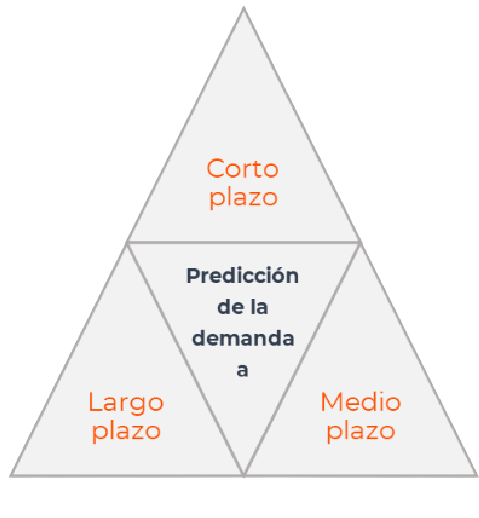
\includegraphics[scale=0.50]{./trianguloCMD.png}
    \caption{Predicción de demanda a corto, mediano y largo plazo.}
    \label{fig:proceso_inventario}
  \end{center}
\end{figure}

\begin{enumerate}
  \item Utiliza la \textbf{Predicción de la demanda a largo plazo para la planificación
          estrategica.} Simula y compara diferentes escenarios hipotéticos de demanda,
        anticipa los cambios de mercado y planifica la contratación futura de recursos.
  \item Utiliza la \textbf{Predicción de la demanda a corto plazo para la planificación
          operativa.} Planifica semanalmente las operaciones y recursos del día.
  \item Utiliza la\textbf{Predicción de la demanda a medio plazo para la planificación
          táctica.} Conoce las capacidades con meses de antelacion y compáralas con las
        actuales para detectar posibles necesidades.
\end{enumerate}
\vspace{1\baselineskip}
La predicción de compra de insumos es vital para la planificación a corto, mediano y largo plazo en un negocio gastronómico por varias razones:

\begin{enumerate}
  \item \textbf{Optimización de Inventario:} El inventario tiene como propósito fundamental proveer a la empresa de materiales necesarios, para  su  continuo  y  regular  desenvolvimiento,  es  decir,  el  inventario  tiene  un  papel  vital  para  el funcionamiento acorde y coherente dentro del proceso de producción y de esta forma afrontar la demanda\cite{marques2017nivel}.

        Al prever la demanda futura, el negocio puede mantener un nivel de inventario
        óptimo. Comprar en exceso puede llevar al desperdicio de alimentos, mientras
        que comprar muy poco puede resultar en escasez y pérdida de ventas.

        \begin{figure}[H]
          \begin{center}
            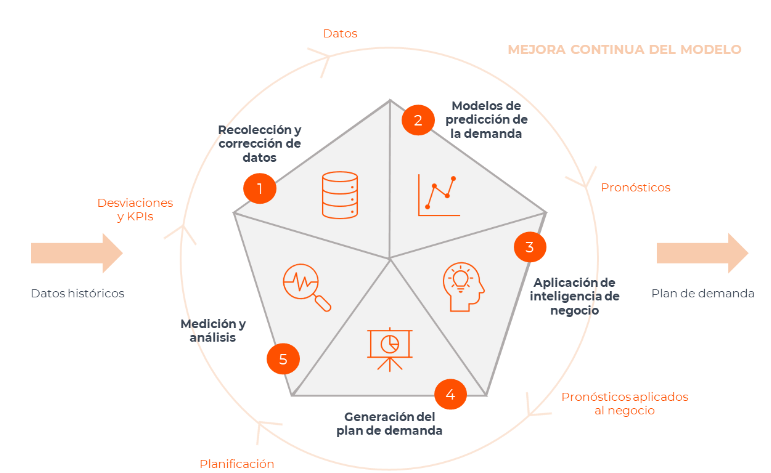
\includegraphics[scale=0.70]{./procesos_de_trabajo.png}
            \caption{Proceso de Optimización de inventario.}
            \label{fig:proceso_inventario}
          \end{center}
        \end{figure}

  \item \textbf{Reducción de Costos:} Una predicción precisa permite comprar solo lo necesario, lo que reduce los costos asociados con el almacenamiento y la conservación de productos perecederos.

        Si se mantienen inventarios demasiado altos, el costo podría llevar a una
        empresa a tener problemas de liquidez financiera, esto ocurre porque un
        inventario “parado” inmoviliza recursos que podrían ser mejor utilizados en
        funciones más productivas de la organización\cite{marques2017nivel}.

  \item \textbf{Eficiencia Operativa:} Saber qué insumos se necesitarán en el futuro permite planificar y programar las operaciones de manera más eficiente, evitando retrasos y problemas logísticos.

        Es útil mantener los inventarios en las empresas porque, se tiene en cuenta la
        capacidad de predicción con el fin de planear la capacidad y establecer un
        cronograma de producción, también fluctuaciones en la demanda ósea una reserva
        de inventarios a la mano que supone protección, inestabilidad de los
        suministros, protección deprecios, descuentos por cantidad, menores costos de
        pedidos\cite{marques2017nivel}.

  \item \textbf{Satisfacción del Cliente:} Mantener un suministro constante de productos esencial para el negocio, ya que los clientes esperan encontrar su elección preferida en el menú en todo momento.
\end{enumerate}

\subsection{Factores que Influyen en la Curva de Insumos Demandados}

Varios factores pueden influir en el comportamiento de la curva de insumos
demandados:

\begin{itemize}
  \item Día de la Semana y Estacionalidad: Los patrones de consumo pueden variar según
        el día de la semana y la temporada. Por ejemplo, los fines de semana pueden
        tener una mayor demanda en comparación con los días laborables.

  \item Eventos Especiales: Eventos como días festivos, celebraciones locales o
        conciertos cercanos pueden aumentar la demanda de alimentos y bebidas.

  \item Tendencias de Consumo: Las tendencias gastronómicas y las preferencias
        cambiantes de los consumidores pueden afectar la demanda de ciertos productos.

  \item Clima: Las condiciones climáticas también pueden influir en la demanda. Por
        ejemplo, un día caluroso podría aumentar la demanda de bebidas frías.

  \item Promociones y Ofertas: Las promociones especiales pueden aumentar temporalmente
        la demanda de ciertos productos.
\end{itemize}

\section{Tiempos Actuales en las Predicciones de Demanda}

En la actualidad, las predicciones de demanda se benefician ampliamente de las
tecnologías avanzadas y el análisis de datos. Las empresas pueden aprovechar
sistemas de gestión de inventario y software de análisis de datos para
recopilar y procesar información histórica y en tiempo real. Estas herramientas
les permiten aplicar técnicas estadísticas y modelos de pronóstico para
anticipar con mayor precisión los patrones de demanda futura.

En tiempos recientes, se ha observado la aplicación de diversas técnicas en el
campo de la inteligencia artificial, como sistemas expertos, y más
recientemente, algoritmos genéticos. Sin embargo, a pesar de esta evolución,
los modelos que han captado una atención destacada son los basados en Redes
Neuronales Artificiales (RNAs). Con el transcurso del tiempo, se han
desarrollado múltiples arquitecturas de RNAs para abordar una variedad de
problemas en el ámbito de la predicción de demanda.

\section{Sistema de información }

Según\cite{kendall2005analisis} el sistema de información\textit{ “Es un
  conjunto de elementos que interactúan entre sí, con el fin de apoyar las
  actividades de una empresa o negocio”}.

Es importante tener en cuenta que la necesidad de información en las
organizaciones es vital para alcanzar el éxito y que un sistema de información
debe justificar su implementación desde el punto de vista costo/beneficio,
basándose en el valor que se le otorga a la información dentro de la
organización \cite{kendall2005analisis}. Los beneficios pueden ser tangibles e
intangibles, y dependen de los objetivos y necesidades de la organización.

\vspace{1\baselineskip}
Los sistemas de información se desarrollan para diferentes propósitos, según las necesidades de los usuarios humanos y la empresa. En definitiva, el uso adecuado de la información y la implementación de sistemas de información efectivos pueden marcar una gran diferencia en el éxito de una organización.

\vspace{1\baselineskip}
\textbf{ Tipos de sistema de información}

El propósito de un sistema de información, puede ser muy amplio, todo depende
de las necesidades de la organización. Existen distintos tipos de sistemas de
información, entre los que destacan los siguientes\cite{kendall2005analisis}:

\setcounter{secnumdepth}{3}
\begin{itemize}

  \item \textbf{Sistemas de procesamiento de transacciones}

        Se define como transacción un suceso que implica o afecta a una organización, y
        que está compuesta por datos referentes a ellas y que son de importancia para
        la organización\cite{kendall2005analisis}. Estos sistemas se encargan del
        procesamiento de los datos referentes a las transacciones, además de permitir
        la automatización de tareas y procesos operativos.

        \vspace{1\baselineskip}
        La información que se obtiene como salida es utilizada posteriormente por los
        funcionarios de nivel operativo de la organización en la toma de decisiones.

        Las razones para el procesamiento de las transacciones son:

        \begin{itemize}
          \item Clasificación: Implica agrupar todos los datos de acuerdo con características
                comunes.
          \item Operaciones de cálculo: Consiste en realizar alguna operación para obtener
                resultados útiles.
          \item Ordenamiento: Consiste en disponerlos de alguna forma o secuencia, facilita el
                procesamiento y la búsqueda.
          \item Síntesis: Reduce los datos en información breve y concisa.
          \item Almacenamiento: Permite el registro de todas y cada una del suceso que afectan
                a la organización.

        \end{itemize}

  \item \textbf{Sistema de información administrativa}

        Los sistemas de información administrativa (MIS) no sustituyen a los sistemas
        de procesamiento de transacciones; más bien, todos los sistemas MIS incluyen el
        procesamiento de transacciones\cite{kendall2005analisis}. Los MIS son sistemas
        de información computarizados que funcionan debido a la decidida interacción
        entre las personas y las computadoras.

        \vspace{1\baselineskip}
        Al requerir que las personas, el software y el hardware funcionen en concierto,
        los sistemas de información administrativa brindan soporte a los usuarios para
        realizar un espectro más amplio de tareas organizacionales que los sistemas de
        procesamiento de transacciones, incluyendo los procesos de análisis y toma de
        decisiones. Para acceder a la información, los usuarios del sistema de
        información administrativa comparten una base de datos común; esta almacena
        tanto los datos como los modelos que permiten al usuario interactuar con ellos,
        interpretarlos y aplicarlos. Los sistemas de información administrativa
        producen información que se utiliza en el proceso de toma de decisiones.
        También pueden ayudar a integrar algunas de las funciones de información
        computarizadas de una empresa.

  \item \textbf{Sistema de soporte de decisiones DSS}

        Son sistemas de información que tienen como propósito auxiliar al usuario con
        las decisiones únicas que no se repiten y que no tienen una estructura
        definida\cite{kendall2005analisis}. Además de estar hechos a la medida de la
        persona o grupo que los usa en comparación con los Sistemas de información
        Gerencial. El propósito de estos sistemas es el de responder correctamente a
        condiciones inesperadas y propias de la información. Esto permite que sean
        empleados en niveles altos de la organización.

  \item \textbf{Sistema de información gerencial}

        Los Sistemas de Información Gerencial, también llamados Sistemas de Reportes de
        Gerencia, se dedican al apoyo de decisiones siempre que los requerimientos de
        información sean identificados, esto es, que la información que necesita para
        la toma de decisiones haya sido analizada anteriormente, y que esta misma
        decisión pueda tomarse nuevamente\cite{kendall2005analisis}. Estos sistemas
        pueden extraer la información necesaria de cualquier parte de la organización,
        por lo que la información necesaria ya se tiene almacenada al ser procesada por
        un sistema de transacciones.

  \item \textbf{Sistema experto e inteligencia artificial }

        La inteligencia artificial (IA) puede ser considerada como el campo dominante
        de los sistemas expertos. La idea general de la IA ha sido desarrollar equipos
        que se comporten de manera inteligente\cite{kendall2005analisis}.

        Dos ramas de investigación de la IA son:

        \begin{itemize}

          \item La comprensión del lenguaje natural.
          \item El análisis de la habilidad para razonar un problema y llegar a una conclusión
                lógica.

        \end{itemize}

        Los sistemas expertos utilizan las metodologías de razonamiento de la IA para
        resolver los problemas que los usuarios de negocios (y otros tipos de usuarios)
        les presentan. Los sistemas expertos son una clase muy especial de sistema de
        información que ha demostrado su utilidad comercial gracias a la disponibilidad
        extendida de hardware y software como las computadoras personales (PC) y las
        interfaces de sistemas expertos.

        \vspace{1\baselineskip}
        Un sistema experto (también conocido como sistema basado en el conocimiento)
        captura y utiliza en forma efectiva el conocimiento de uno o varios expertos
        humanos para resolver un problema específico al que una organización se
        enfrenta. Cabe mencionar que a diferencia de los sistemas DSS, que en última
        instancia dejan la decisión a la persona encargada de la toma de decisiones, un
        sistema experto selecciona la mejor solución para un problema o una clase
        específica de problemas. Los componentes básicos de un sistema experto son la
        base de conocimiento, un motor de inferencia que conecta al usuario con el
        sistema mediante el proceso de consultas en lenguajes, como el lenguaje de
        consulta estructurado (SQL), y la interfaz de usuario. Las personas conocidas
        como ingenieros del conocimiento capturan la experiencia de los expertos, crean
        un sistema computacional que incluye este conocimiento y después lo
        implementan\cite{kendall2005analisis}.

        \begin{figure}[H]
          \begin{center}
            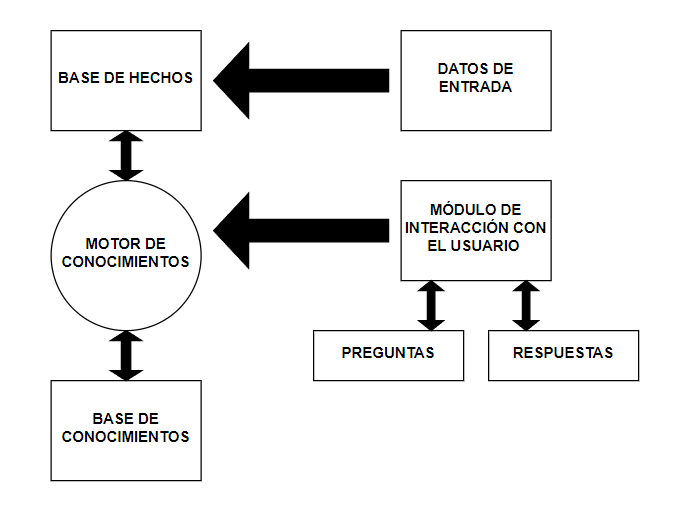
\includegraphics[scale=0.70]{./hechos.png}
            \caption{Arquitectura de un sistema experto.}
            \label{fig:Arquitectura de un sistema experto}
          \end{center}
        \end{figure}

        En los Sistemas Expertos el conocimiento se hace explícito en forma de reglas,
        en la computación neuronal las ANN generan sus propias reglas aprendiendo de
        los ejemplos que se les muestran en la fase de
        entrenamiento\cite{olabe1998redes}.

\end{itemize}

\section{Mineria de datos}
La minería de datos puede definirse inicialmente como un proceso de
descubrimiento de nuevas y significativas relaciones, patrones y tendencias al
examinar grandes cantidades de datos\cite{perez2007mineria}.

\vspace{1\baselineskip}
El análisis de datos, potenciado por herramientas informáticas, ha dado lugar a la minería de datos. Esta disciplina busca descubrir automáticamente conocimiento en grandes bases de datos, identificando patrones, tendencias y perfiles a través de tecnologías avanzadas como el reconocimiento de patrones, redes neuronales y algoritmos genéticos.

\vspace{1\baselineskip}
Inicialmente, los sistemas de información se centraban en recopilar datos para apoyar la toma de decisiones. Con la informatización de las organizaciones, se amplió su función para respaldar los procesos esenciales. Ahora, se buscan
prestaciones adicionales, como sistemas de información para la toma de decisiones.

\vspace{1\baselineskip}
La Minería de Datos se puede ubicar en el nivel más alto de la evolución de los procesos tecnológicos de análisis de datos \cite{martinez2001mineria}.

\vspace{1\baselineskip}
La Minería de Datos involucra e integra técnicas de diferentes disciplinas tales como tecnologías de bases de datos y data warehouse, estadística, aprendizaje de máquina, computación de alta performance, com  putación evolutiva, reconocimiento de patrones, redes neuronales, visualización de datos, recuperación de información, procesamiento de imágenes y señales, y análisis de datos espaciales o temporales\cite{schab2018mineria}.

\section{Técnicas de modelado de procesos de ETL}

Las herramientas de Extracción-Transformación-Carga (ETL) son piezas de
software responsables de la extracción de datos de varias fuentes, su limpieza,
personalización e inserción en un almacén de datos\cite{SIMITSIS200822}.

\vspace{1\baselineskip}
El proceso de extracción, transformación y carga – ETL es una de las actividades técnicas más críticas en el desarrollo de soluciones de inteligencia de negocios BI \cite{martinez2013tecnicas}.

\vspace{1\baselineskip}
El proceso de ETL es esencial para garantizar la calidad y la integridad de los datos antes de que se utilicen en aplicaciones analíticas o de toma de decisiones. Permite a las organizaciones transformar datos crudos en información procesable y confiable. Además, con la creciente cantidad de datos disponibles en la actualidad, el ETL se ha vuelto cada vez más importante para integrar datos de diversas fuentes y garantizar que estén listos para su análisis.

\vspace{1\baselineskip}
Para autores como Ralph Kimball los Almacenes de Datos son “una copia de los datos transaccionales estructurados específicamente para consultas y análisis”, mientras que Bill Inmon define el término Almacén de Datos como: “una colección
de datos orientados por temas, integrados, variables en el tiempo y no volátiles para el apoyo de la toma de decisiones”. Los Almacenes de Datos son integradores, ya que su contenido proviene de diversas fuentes de datos como:
Sistemas heredados, Archivos de Textos, Base de Datos Relacionales, ERP, entre otras posibilidades. La forma de lograr esta integración es a través del uso y desarrollo de los Procesos ETL. Estos procesos son los encargados de la extracción de los datos desde sus fuentes de origen, de transformarlos a la información deseada, de lograr la limpieza necesaria en aquellos que lo requieran y finalmente cargar al Almacén de Datos deseado, el que será utilizado con alguna finalidad como análisis en un área de las ventas de una
corporación o el estudio de tendencias de alguna
consultora\cite{villarroel2013incorporacion}.

\section{Inteligencia Artificial}
\subsection{El aprendizaje automático \textit{(machine learning)}}

El aprendizaje automático como area de las ciencias computacionales aplicadas,
desarrolla algoritmos capaces de tomar datos numéricos y alfanuméricos
almacenados en un computador\cite{herrera2020prediccion}.

\vspace{1\baselineskip}
\textit{Según Arthur Samuel, el aprendizaje automático se define como el campo de estudio que otorga a las computadoras la capacidad de aprender sin ser programadas explícitamente}\cite{mahesh2020machine}. Es decir en lugar de seguir instrucciones detalladas, las computadoras pueden mejorar su desempeño mediante la adquisición de conocimiento y habilidades a partir de datos y experiencias previas

\vspace{1\baselineskip}
El aprendizaje automático se utiliza para enseñar a las máquinas a manejar los datos de manera más eficiente. A veces, después de ver los datos, no podemos interpretar la información extraída de los mismos. En ese caso, aplicamos el aprendizaje automático.

\vspace{1\baselineskip}
Con la abundancia de conjuntos de datos disponibles, la demanda de aprendizaje automático está en aumento. Muchas industrias aplican el aprendizaje automático
para extraer datos relevantes. El propósito del aprendizaje automático es aprender de los datos. Se han realizado muchos estudios sobre cómo hacer que las máquinas aprendan por sí mismas sin ser programadas explícitamente. Muchos matemáticos y programadores aplican varios enfoques para encontrar la solución a este problema que implica conjuntos de datos enormes\cite{mahesh2020machine}.

\vspace{1\baselineskip}
El Aprendizaje Automático se basa en diferentes algoritmos para resolver problemas de datos. A los científicos de datos les gusta señalar que no existe un único tipo de algoritmo que sea universal y mejor para resolver todos los problemas. El tipo de algoritmo utilizado depende del tipo de problema que se desee resolver, el número de variables, el tipo de modelo que se adapte mejor, entre otros factores.

\vspace{1\baselineskip}
Las técnicas de machine learning son necesarias para mejorar la precisión de
los modelos predictivos. Dependiendo de la naturaleza del problema empresarial
que se está atendiendo, existen diferentes enfoques basados en el tipo y
volumen de los datos\cite{ibm}.

\vspace{1\baselineskip}
Una forma común de describir a un conjunto de datos u observaciones (dataset)
es con una matriz de diseño. Una matriz de diseño es una matriz que contiene un
ejemplo diferente en cada fila. Cada columna de la matriz corresponde a una
característica diferente. Los algoritmos de aprendizaje se diferencian en
función de la forma de operar y procesa los datos contenidos en una matriz de
diseño\cite{arana2021redes}.

\vspace{1\baselineskip}
En el contexto de la aplicación de algoritmos de Machine Learning en el cálculo
de pronósticos de demanda, es esencial comprender que el objetivo principal de
estos algoritmos es encontrar una función que tome un conjunto de variables
como entrada y produzca una estimación del valor deseado, en este caso, la
demanda. Esta función se ajusta a través del aprendizaje a partir de
observaciones pasadas donde los datos de demanda son conocidos. Por ejemplo,
utilizando datos de demanda de los últimos años, el modelo se entrena para
desarrollar una función que pueda hacer predicciones precisas sobre la demanda
futura, lo que implica una tarea de regresión, ya que el resultado esperado es
un valor numérico real. Esta metodología se basa en el libro “Deep Learning” de
Ian Goodfellow, Yoshua Bengio y Aaron Courville\cite{goodfellow2016deep}.

\vspace{1\baselineskip}
El siguiente diagrama muestra un flujo de trabajo típico para el uso del
aprendizaje automático en modelado predictivo \cite{mirjalili2020python}:

\begin{figure}[H]
  \begin{center}
    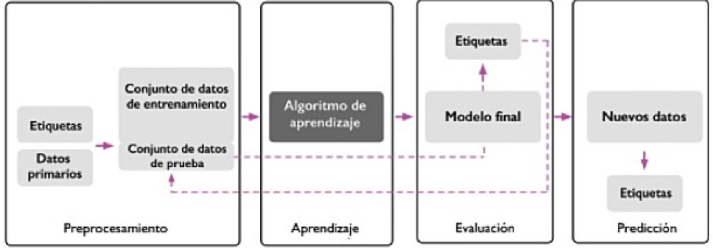
\includegraphics[scale=0.80]{./uso_aprendisaje_automatico.png}
    \caption{ flujo de trabajo típico para el uso del aprendizaje automático en modelado predictivo}
    \label{fig:perceptron}
  \end{center}
\end{figure}
\begin{itemize}
  \item \textbf{Procesamiento:}
        \begin{itemize}
          \item Extracción y escalado de características.
          \item Selección de características.
          \item Reducción de la dimensionalidad.
          \item Muestreo.
        \end{itemize}
  \item \textbf{Aprendizaje:}
        \begin{itemize}
          \item Selección del modelo.
          \item Validación cruzada.
          \item Medición del rendimiento.
          \item Optimización de hiperparametro.
        \end{itemize}
\end{itemize}
\subsection{Aprendizaje supervisado}

El aprendizaje supervisado comienza típicamente con un conjunto establecido de
datos y una cierta comprensión de cómo se clasifican estos datos. El
aprendizaje supervisado tiene la intención de encontrar patrones en datos que
se pueden aplicar a un proceso de analítica. Estos datos tienen características
etiquetadas que definen el significado de los datos. Por ejemplo, se puede
crear una aplicación de machine learning con base en imágenes y descripciones
escritas que distinga entre millones de animales\cite{ibm}.

\vspace{1\baselineskip}
El objetivo principal del aprendizaje supervisado es aprender un modelo, a partir de datos de entrenamiento etiquetados, que nos permite hacer predicciones sobre datos futuros o no vistos \cite{mirjalili2020python}. Aquí, el término supervisado se refiere a un conjunto de muestras donde las señales
de salida deseadas (etiquetas) ya se conocen.

\begin{figure}[H]
  \begin{center}
    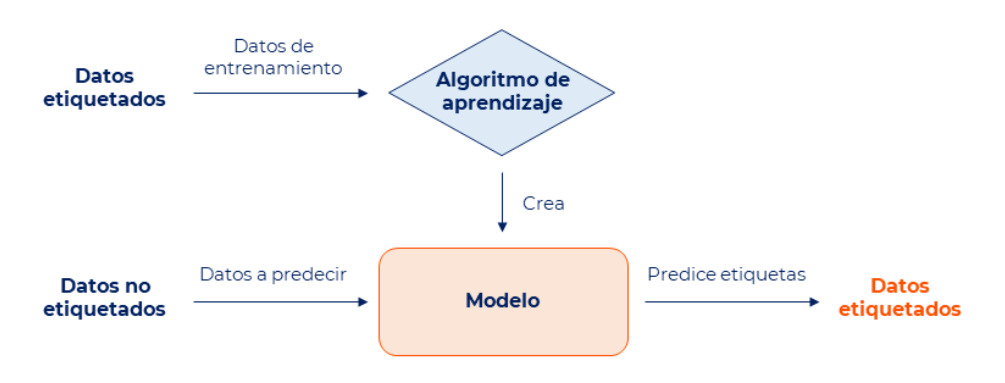
\includegraphics[scale=0.60]{./aprendisaje_supervisado.png}
    \caption{Aprendisaje supervisado.}\cite{decide}
    \label{fig:aprendisajesupervisado}
  \end{center}
\end{figure}

\subsection{Aprendizaje no supervisado}

El aprendizaje no supervisado se utiliza cuando el problema requiere una
cantidad masiva de datos sin etiquetar. Por ejemplo, las aplicaciones de redes
sociales, tales como Twitter, Instagram y Snapchat, tienen grandes cantidades
de datos sin etiquetar. La comprensión del significado detrás de estos datos
requiere algoritmos que clasifican los datos con base en los patrones o
clústeres que encuentra. El aprendizaje no supervisado lleva a cabo un proceso
iterativo, analizando los datos sin intervención humana\cite{ibm}.

Los métodos de aprendizaje no supervisados son utilizados durante el
preprocesamiento de los datos antes de ser utilizados por algoritmos de
característica supervisada. Estos algoritmos también son muy utilizados en la
compresión de datos. Todos los métodos son implícita o explícitamente basados
en la distribución de probabilidad en el espacio definido por las variables de
entrada\cite{de2014aprendizaje}.

\subsection{Aprendizaje de refuerzo}

El aprendizaje de refuerzo es un modelo de aprendizaje conductual. El algoritmo
recibe retroalimentación del análisis de datos, conduciendo el usuario hacia el
mejor resultado. El aprendizaje de refuerzo difiere de otros tipos de
aprendizaje supervisado, porque el sistema no está entrenado con el conjunto de
datos de ejemplo. Más bien, el sistema aprende a través de la prueba y el
error. Por lo tanto, una secuencia de decisiones exitosas conduce al
fortalecimiento del proceso, porque es el que resuelve el problema de manera
más efectiva \cite{ibm}.

\subsection{Redes Neuronales Artificiales}
Las Redes Neuronales Artificiales (RNA) son un componente esencial de la
Inteligencia Artificial que emula el funcionamiento de las neuronas biológicas.
Estas redes, entrenadas con entradas de escenarios internos o externos
multiplicadas por pesos aleatorios, destacan en la resolución de funciones
altamente no lineales, lo que las convierte en herramientas poderosas para la
predicción. Inspiradas en el sistema nervioso biológico, encuentran
aplicaciones en áreas como neurociencias, matemáticas, estadísticas y más. Su
capacidad para aprender de datos de entrada las hace especialmente valiosas en
la predicción de patrones complejos en diversos campos, como finanzas, ciencia
de datos y análisis de mercado. Es un algoritmo basado en una red de alimentación de múltiples capas entrenadas
inspirado en las neuronas del cerebro humano, estos sistemas aprenden y se
forman a sí mismos ya que sus neuronas artificiales están conectadas, en lugar
de ser programados de forma explícita\cite{herrera2020prediccion }.

\vspace{1\baselineskip}
En el desarrollo de una red neuronal no hay que programar ni el conocimiento ni las reglas del procesamiento del conocimiento. La red neuronal aprende las reglas del procesamiento del conocimiento mediante el ajuste de las conexiones ponderadas entre las neuronas de distintas capas de la red.
El aprendizaje se consigue a través de una regla de aprendizaje que adapta o cambia los pesos de las conexiones en respuesta a los ejemplos de entrada, y opcionalmente también en respuesta a las salidas deseadas. Esta característica de las ANN es lo que permite decir que las redes neuronales aprenden de la experiencia\cite{olabe1998redes}.

% \subsection{La Neurona Artificial}
\vspace{1\baselineskip}
La neurona artificial fue diseñada para “emular” las características del funcionamiento básico de la neurona biológica \cite{basogain2008redes}. En esencia, se aplica un conjunto de entradas a la neurona, cada una de las cuales representa una salida de otra neurona . Cada entrada se multiplica por su “peso” o ponderación correspondiente análogo al grado de conexión de la sinapsis. Todas las entradas ponderadas se suman y se determina el nivel de excitación o activación de la neurona.

\vspace{1\baselineskip}
Representación vectorial del funcionamiento básico de una neurona artificial se
indica según la siguiente expresión de la ecuación.

\[
  NET = X \cdot W
\]

Siendo NET la salida, X el vector de entrada y W el vector de pesos.

\vspace{1\baselineskip}
La representación del modelo matemático es el siguiente

\begin{equation}
  y = H\left(\sum_{j=1}^{n} w_jx_j - u\right)
\end{equation}

Donde \(H\) es la función de activación (en este caso la función escalón de
Heaviside) con el umbral \(u\), \(x_j\) es la señal de entrada y \(w_j\) es el
peso asociado con \(j = 1,2,\ldots,n\), donde \(n\) corresponde al número de
entradas. La salida de esta unidad es 1 cuando la suma está por encima del
umbral \(u\), y es 0 en caso contrario\cite{arana2021redes}.

\vspace{1\baselineskip}
El elemento fundamental de los sistemas neuronales biológicos es la neurona, una célula viva que, como tal contiene todos los elementos que integran las células biológicas, si bien incorpora otros elementos que la diferencian. De forma genérica, una neurona consta de un cuerpo celular o soma más o menos esférico (de entre 10 y 80 micras de longitud), del que parten una rama principal o axón (cuya longitud varía desde las 100 micras hasta el metro en el caso de las neuronas motoras que constituyen los nervios) y un denso árbol de ramificaciones más cortas (árbol dendrítico), compuesto por dendritas  (Figura~\ref{fig:componentes}). A su vez, el axón puede ramificarse en su punto de arranque, y con frecuencia presenta múltiples ramas en su extremo. La forma final de la neurona depende de la función que cumple, esto es, de la posición que ocupa en el conjunto del sistema y de los estímulos que recibe \cite{lopez2008redes}.

\begin{figure}[H]
  \begin{center}
    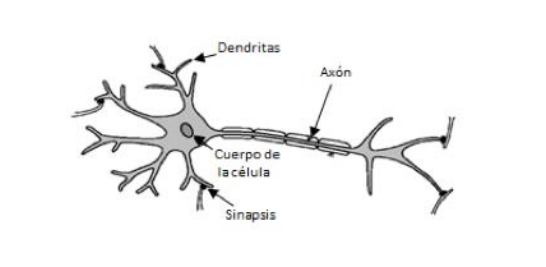
\includegraphics[scale=0.70]{./neuroma_humana.png}
    \caption{Componentes de una neurona.}
    \label{fig:componentes}
  \end{center}
\end{figure}

\subsection{Capas de la neurona artificial}
\textbf{\textit{Desde un punto de vista funcional}}, las neuronas constituyen procesadores de información sencillos, integrados por:
Un canal de recepción de información, las dendritas, que reciben señales de entrada (inputs) procedentes de otras células (interneuronas) o del exterior (neuronas receptoras o sensoras, como los conos y bastones de la retina)\cite{sanchez2015maquinas}.

\vspace{1\baselineskip}
\textbf{\textit{Un órgano de cómputo}}, el soma, que combina e integra los inputs recibidos (generalmente a través de funcionales no lineales), emitiendo señales de salida en forma de estímulos nerviosos\cite{sanchez2015maquinas}.

\vspace{1\baselineskip}
\textbf{\textit{Un canal de salida}}, el axón, que envía la salida generada por el soma a
otras neuronas o bien, en el caso de las neuronas motoras, directamente al
músculo. Para transmitir la información, el axón se conecta a través de sus ramificaciones a las dendritas de otras neuronas, que reciben las señales y las combinan para producir nuevas salidas. Una neurona del córtex cerebral recibe información, por término medio, de unas 10.000 neuronas (convergencia), y envía impulsos a varios cientos de ellas (divergencia)\cite{sanchez2015maquinas}.

\begin{figure}[H]
  \begin{center}
    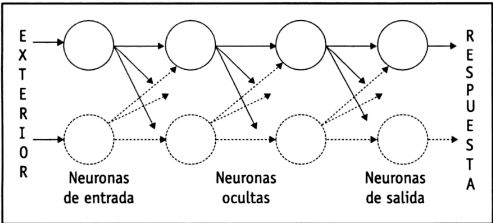
\includegraphics[scale=0.90]{./tipo_neuronas.png}
    \caption{Tipos de neuronas artificiales.}\cite{lopez2008redes}
    \label{fig:tipo}
  \end{center}
\end{figure}

Caracteristicas de tres tipos de neuronas artificiales: unidades de entrada, de
salida y unidades ocultas(Figura~\ref{fig:tipo})\cite{lopez2008redes}.

\begin{itemize}
  \item  Las neuronas de entrada reciben señales desde el entorno, provenientes de
        sensores o de otros sectores del sistema (como archivos de almacenamiento de
        patrones de aprendizaje).

  \item Las neuronas de salida envían su señal directamente fuera del sistema una vez
        finalizado el tratamiento de la información (salidas de la red).

  \item Las neuronas ocultas reciben estímulos y emiten salidas dentro del sistema, sin
        mantener contacto alguno con el exterior. En ellas se lleva a cabo el
        procesamiento básico de la información, estableciendo la representación interna
        de ésta.
\end{itemize}

\subsection{Modelo de redes neuronales artificiales}

Las redes neuronales artificiales son motivadas por ciertas cualidades de su
modelo real, por lo cual el desafio es producir un modelo que tenga
\cite{nacelle2009redes}:
\begin{itemize}
  \item  Una estructura de procesamiento distribuida y paralela (opuestamente al CPU de una comutadora).

        % La arquitectura de las ANN parte de la organización de los sistemas de procesado en paralelo, es decir, sistemas en los que distintos procesadores están interconectados. No obstante los procesadores son unidades procesadoras simples, diseñadas para la suma de muchas entradas y con un ajuste automático de las conexiones ponderadas.

  \item Alto grado de conexion entre las unidades basicas.
  \item Conexiones modificables en funcion de la experiencia.
  \item Un proceso de aprendizaje constante y de ser posible uno no supervisado.
  \item Aprendisaje basado en informacion local.
  \item Robustez en la performance si algunas unidades son removidas.

\end{itemize}

\subsection{Arquitectura de una red neuronal}
La topotogia o arquitectura hace referencia a la organización y disposición de
las neuronas en la red formando capas de procesadores interconectados entre sí
a través de sinapsis unidireccionales. La arquitectura de una RNA depende de
cuatro parámetros principales \cite{lopez2008redes}:

\begin{itemize}
  \item el número de capas,
  \item el número de neuronas por capa,
  \item el grado de conectividad entre las neuronas y
  \item el tipo de conexiones neuronales.
\end{itemize}

\vspace{1\baselineskip}
Las arquitecturas neuronales pueden clasificarse atendiendo a distintos criterios \cite{lopez2008redes}:

\begin{itemize}
  \item Según su estructura en capas
        \begin{itemize}
          \item Redes monocapa, compuestas por una única capa de neuronas, entre las que se
                establecen conexiones laterales y, en ocasiones, autorrecurrentes. Este tipo de
                redes suele utilizarse para la resolución de problemas de autoasociación y
                clusterización.

          \item Redes multicapa (layered networks), cuyas neuronas se organizan en varias capas
                (de entrada, oculta(s) y de salida). La capa a la que pertenece la neurona
                puede distinguirse mediante la observación del origen de las señales que recibe
                y el destino de la señal que genera.
        \end{itemize}

  \item Según el flujo de datos en la red

        \begin{itemize}
          \item Redes unidireccionales o de propagación hacia adelante (feedforward), en las
                que ninguna salida neuronal es entrada de unidades de la misma capa o de capas
                precedentes. La información circula en un único sentido, desde las neuronas de
                entrada hacia las neuronas de salida de la red.

          \item Redes de propagación hacia atrás (feedback), en las que las salidas de las
                neuronas pueden servir de entradas a unidades del mismo nivel (conexiones
                laterales) o de niveles previos. Las redes de propagación hacia atrás que
                presentan lazos cerrados se denominan sistemas recurrentes.
        \end{itemize}
\end{itemize}
\subsection{Perceptron}
En 1957, Frank Rosenblatt publicó el mayor trabajo de investigación en
computación neuronal realizado hasta esas fechas. Su trabajo consistía en el
desarrollo de un elemento llamado “Perceptron” \cite{olabe1998redes}.

\vspace{1\baselineskip}
El perceptron es un sistema clasificador de patrones que puede identificar patrones geométricos y abstractos. El primer perceptron era capaz de aprender algo y era robusto, de forma que su comportamiento variaba sólo si resultaban dañados los componentes del sistema.
Además presentaba la característica de ser flexible y comportarse correctamente después de que algunas celdas fueran destruidas.
El perceptron fue originalmente diseñado para el reconocimiento óptico de patrones. Una rejilla de 400 fotocélulas, correspondientes a las neuronas de la retina sensibles a la luz, recibe el estímulo óptico. Estas fotocélulas están conectadas a elementos asociativos que recogen los impulsos eléctricos emitidos desde las fotocélulas. Las
conexiones entre los elementos asociativos y las fotocélulas se realizan de forma aleatoria.
Si las células presentan un valor de entrada superior a un umbral predeterminado entonces el elemento asociativo produce una salida\cite{olabe1998redes}.

\begin{figure}[H]
  \begin{center}
    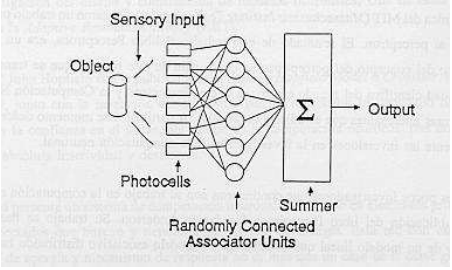
\includegraphics[scale=0.90]{./perceptron.png}
    \caption{Aplicación de la Red Perceptron}
    \label{fig:perceptron}
  \end{center}
\end{figure}

\subsection{Perceptrón multica}
Una Perceptrón multicapa (MLP) puede ser interpretada como una extensión del algoritmo de regresión logística donde primero la entrada es transformada utilizando una transformación no lineal\cite{de2014aprendizaje}. El propósito de esta transformación es proyectar los datos de entrada a un espacio donde sean linealmente separables. Esta capa intermedia es conocida como capa oculta y es característica de una MLP poseer dos o mas de ellas. Una capa oculta única es suficiente para hacer de una MLP un aproximador universal.

\subsection{Redes neuronales recurrentes (RNN)}

Una de las ideas principales que propició el desarrollo de estas redes fue
extraída de las técnicas de aprendizaje automático y de los modelos
estadísticos encontrados en la década de los 80. Esta idea se basaba en
compartir diferentes parámetros a lo largo de diferentes partes de un modelo. Esto permitió generalizar conjuntos de datos que contaban con dependencias temporales entre sus entradas \cite{Goodfellow-et-al-2016}.

\vspace{1\baselineskip}
Un perceptrón multicapa tendría muy difícil el hecho de generalizar sobre una secuencia debido a que, si entrenamos esta red con secuencias de longitud fija, la red tendría parámetros separados para cada una de las características de entrada teniendo que aprender todas las reglas por separado. Sin embargo, la RNNs encontraría esta tarea mucho más fácil debido a que comparte pesos a lo largo del tiempo. Cabe mencionar que cuando mencionamos el tiempo no tiene por que significar literalmente tiempo, puede simplemente significar la posición de un objeto en una secuencia \cite{roman2018redes}.

\vspace{1\baselineskip}
Las redes neuronales recurrentes tienen caminos de retroalimentación entre
todos los elementos que las conforman. Una sola neurona está entonces conectada a las neuronas posteriores en la siguiente capa, las neuronas pasadas de la capa anterior y a ella misma a través de vectores de pesos variables que sufren alteraciones en cada época con el fin de alcanzar los parámetros o metas de operación\cite{montesdeoca2016estudios}.

\vspace{1\baselineskip}
Las redes neuronales recurrentes (RNNs) son un tipo de modelo de aprendizaje profundo que se utiliza para analizar datos secuenciales, como el procesamiento del lenguaje natural o la predicción de series de
tiempo\cite{tomas2023prediccion}.

\vspace{1\baselineskip}
A diferencia de las redes neuronales artificiales ya vistas, que asumen la
independencia entre los datos de entrada, las \gls{rnn} capturan activamente sus dependencias secuenciales y temporales\cite{arana2021redes}.

\vspace{1\baselineskip}
Las RNN generalmente aumentan la arquitectura de red multicapa convencional con la adición de ciclos que conectan nodos adyacentes o pasos de tiempo.  Estos ciclos constituyen la memoria interna de la red que se utiliza para
evaluar las propiedades del dato actual con respecto a los datos del pasado
inmediato. Las redes neuronales recurrentes son más eficaces para resolver problemas con no ­linealidades temporales significativas. Son especialmente útiles en aplicaciones tales como el reconocimiento de patrones secuenciales, cambiantes en el tiempo, ya que las capacidades de predicción y mapeo de las RNN así lo permiten\cite{montesdeoca2016estudios}.

\vspace{1\baselineskip}
Sin embargo, la capacidad de las RNNs para manejar datos a largo plazo se ve comprometida por el problema del gradiente que desaparece, que ocurre cuando el gradiente se hace cada vez más pequeño a medida que se propaga hacia atrás en la red. Para superar este problema, Hochreiter \& Schmidhuber, propusieron la memoria a corto y largo plazo (LSTM), una variante de las RNNs que ha demostrado ser efectiva para el procesamiento de datos secuenciales a largo plazo\cite{tomas2023prediccion}.

\subsection{Arquitectura básica de una RNN}
Arquitectura básica de una RNN. Una característica importante es la inclusión de retrasos ($z^{-1}$) a la salida de las neuronas en las capas intermedias.

% \vspace{1\baselineskip}
% Los retrasos ($z^{-1}$) se refieren a la retroalimentación de la salida de una neurona en un instante de tiempo anterior como una entrada en el instante de tiempo actual. Esto significa que una RNN puede mantener y usar información de las entradas anteriores en su procesamiento actual. Esto es especialmente útil en problemas donde la secuencia de datos es importante y la información previa es relevante para la predicción o clasificación actual.

\vspace{1\baselineskip}
Las salidas parciales $S_{mn}(t + 1)$ se convierten en valores $S_{mn}(t)$, un instante de tiempo anterior, y así se retroalimenta a todos los componentes de la red, guardando información de instantes de tiempo anteriores \cite{montesdeoca2016estudios}.Se puede apreciar cómo todos los nodos están interconectados entre sí, estableciendo conexiones tanto directas como mediante retardos temporales con los nodos precedentes en cada capa, lo que permite la incorporación de memorias temporales.

\begin{figure}[H]
  \begin{center}
    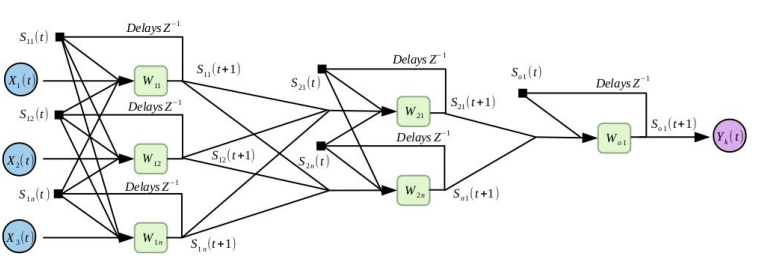
\includegraphics[scale=0.70]{./redes_recurrentes.png}
    \caption{La arquitectura básica de una RNN}
    \label{fig:red_recurreente}
  \end{center}
\end{figure}

\newacronym{lstm}{LSTM}{Redes de Memoria Corta y Larga}
\glsreset{lstm} % reinicia el banderín del primer uso

\subsection{Redes de Memoria Corta y Larga  LSTM}

Las redes de “larga memoria de corto plazo”(\gls{lstm}), propuestas por
Hochreiter y Schmidhuber. Es una de las arquitecturas de aprendizaje profundo más avanzadas y exitosas para predicción de series temporales, reconocimiento de escritura y análisis de discurso\cite{fernandez2021estimacion}.

\vspace{1\baselineskip}
El modelo matemático de LSTM se define como una función no lineal que
transforma la entrada actual, el estado anterior y la memoria a largo plazo en una salida y un estado actualizado.

\vspace{1\baselineskip}
El cálculo de esta función implica la operación de multiplicación de matrices y
la aplicación de funciones de activación, como la función sigmoide o la
tangente hiperbólica\cite{tomas2023prediccion}.

% \vspace{1\baselineskip}
% El objetivo es mejorar la memoria de la RNN de los eventos pasados entrenándola
% para que recuerde lo importante y olvide el resto. Para ello, las LSTM procesan
% dos versiones del pasado \cite{arana2021redes}.

% \vspace{1\baselineskip}
% Las LSTM's Estas se han diseñado para evaluar series de datos donde el pasado
% es importante para presentar una evaluación futura.tienen un alta sensibilidad
% a los datos a escala en entrada, más aún cuando las funciones de activación son
% la tangente hiperbólicaro la función sigmoidea. Debido a esto es necesario
% realizar el escalado de los datos \cite{escobar2022evaluacion}.

\vspace{1\baselineskip}
Las unidades LSTM (Long Short-Term Memory) son unidades utilizadas en la construcción de redes recurrentes. Cada unidad LSTM es una celda con cuatro puertas (gates): la input gate, la external input gate, la forget gate y output gate. Lo más importante de la celda es su estado interno, encargado de recordar valores a lo largo del tiempo \cite{roman2018redes}.

\begin{figure}[H]
  \begin{center}
    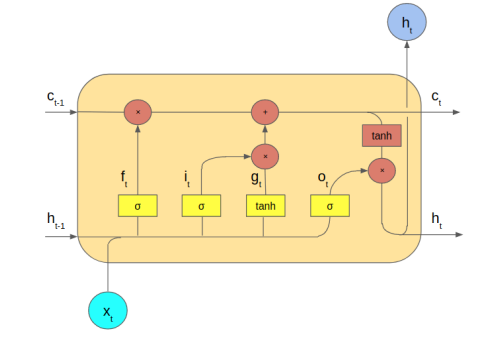
\includegraphics[scale=0.80]{./lstm_grafico.png}
    \caption{Representación de una celda LSTM.}
    \label{fig:lstm_grafico}
  \end{center}
\end{figure}


El \textbf{estado interno} está representado en el diagrama anterior por C y
recorre todas las celdas encadenadas, experimentando pequeños cambios cada vez
que pasa por cada una de ellas.

\vspace{1\baselineskip}
El \textbf{estado oculto} \textit{(hidden-state)} es, sin embargo, la salida de
cada una de las unidades y se comparte a lo largo de todas las unidades de
nuestro modelo. Está representado con la letra h.

\vspace{1\baselineskip}
El primer cambio que experimenta el estado interno es causado por la
forget-gate (ft). Esta puerta decide si el valor presente en el estado de la
celda debe ser olvidado o no \cite{roman2018redes}. Esta decisión se toma
aplicando la función sigmoide sobre la entrada y el estado oculto de la celda
anterior, y multiplicando el resultado por el estado interno proveniente de la
celda anterior. Dado que esta función toma valores entre 0 y 1, puede dar como
resultado 0, lo que significa que se debe olvidar, o dar como resultado 1, lo
que indica que el valor anterior debe ser completamente recordado.

\[f(t) = \sigma \left( b_f + U_f x(t) + W_f h(t-1) \right)\]

\subsection{Modelo de Regresión Lineal}

La siguiente figura \ref{fig:red_recurreente} ilustra el concepto de regresión
lineal. Dada una variable predictora x y una variable de respuesta y, aplicamos
una línea fina a este dato, que minimiza la distancia normalmente, la distancia
cuadrada de promedio entre los puntos de muestra y la línea aplicada. Ahora
podemos utilizar la intersección y la pendiente aprendidas de este dato para
predecir la variable de resultado del nuevo dato\cite{mirjalili2020python}:
\begin{figure}[H]
  \begin{center}
    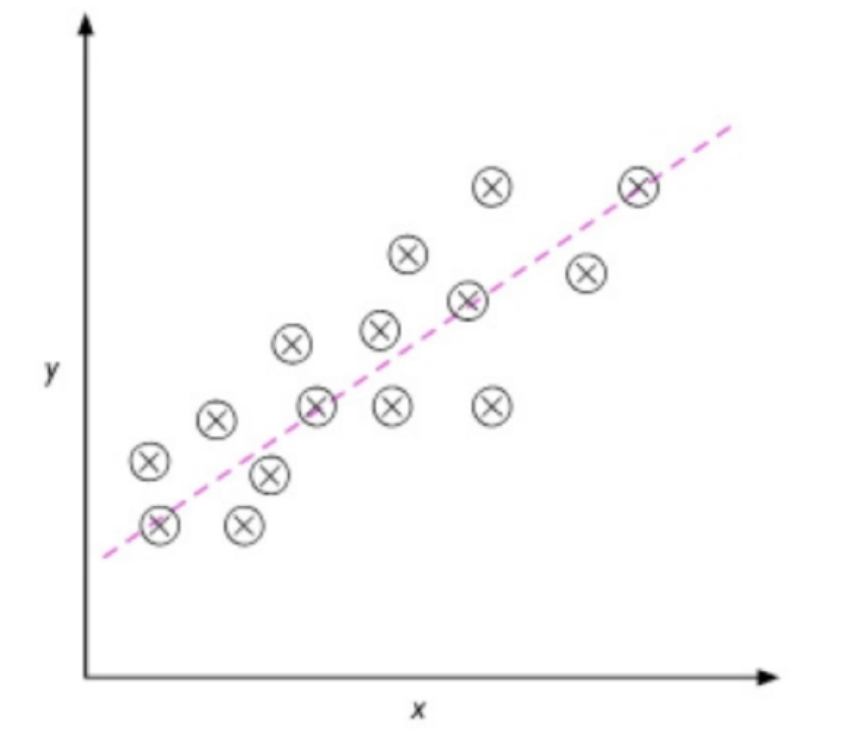
\includegraphics[scale=0.40]{./grafico_regresion.png}
    \caption{Regresión lineal}
    \label{fig:red_recurreente}
  \end{center}
\end{figure}

El modelo de regresión lineal es un método estadístico utilizado para modelar
la relación entre una variable dependiente (la variable que queremos predecir)
y una o más variables independientes (las variables que se utilizan para
predecir la variable dependiente). El objetivo es encontrar una relación lineal
que mejor se ajuste a los datos observados \cite{sepulveda2023analisis}.

\vspace{1\baselineskip}
En general, si se incluyen cada vez más variables en un modelo de regresión, el
ajuste a los datos mejora, aumenta la cantidad de parámetros a estimar pero
disminuye su precisión individual (mayor varianza) y, por tanto, la de la
función de regresión estimada, produciéndose un sobreajuste. Por el contrario,
si se incluyen menos variables de las necesarias en el modelo, las varianzas se
reducen, pero los sesgos aumentarán obteniéndose una mala descripción de los
datos\cite{carrasco2016tecnicas}.

%\cite{chang2023comparacion}
\subsection{Los pesos sinápticos}
A una neurona artificial se le asigna un peso sináptico a las entradas que
provienen desde otras neuronas. Este procedimiento es similar al que se realiza
en una neurona de un ser humano, a lo que normalmente en la medicina se le
conoce como sinapsis. El peso sináptico entonces es un valor numérico y que
puede ir cambiando durante la fase de
entrenamiento\cite{acevedo2017principios}. Este peso hace que la red neural
tengo una utilidad y es allí donde se almacena la información.

En una red de neuronas existe un peso o fuerza sináptica que va a ser un valor
numérico que pondera las señales que se reciben por sus entradas. Este peso
será un valor que determina la fuerza de conexión entre 2 neuronas. Cuando se
evalúa una neurona se debe calcular el conjunto de todas las fuerzas o valores
(denominado NET) que se reciben por sus entradas. Una vez calculado el valor
conjunto de todas las entradas se aplica una función de activación (FA) que
determinará el valor del estado interno de la neurona y que será lo que se
transmita a su salida\cite{pose2009introduccion}.

\section{Métricas para la evaluación de una red neuronal}

\subsection{El error medio cuadrático (MSE) }

El MSE es una medida del error cuadrático medio que se utiliza comúnmente para
evaluar la precisión de un modelo de predicción \cite{sepulveda2023analisis}.
Se define como la media de los errores cuadrados entre los valores observados y
los valores predichos por el modelo. Esta métrica calcula el valor promedio de
los errores elevados al cuadrado\cite{chang2023comparacion}.

La expresión matemática es la siguiente:

\[
  \text{MSE} = \frac{1}{n} \sum_{i=1}^{n} (y_i - \hat{y}_i)^2
\]

Donde:

\begin{itemize}
  \item $n$ : número de observaciones.
  \item $y_i$ : valor observado de la i-ésima observación.
  \item $\hat{y}_i$ : valor predicho por el modelo para la i-ésima observación.
\end{itemize}

\subsection{Raíz del error medio cuadrático (RMSE)}

El RMSE (Error Cuadrático Medio de la Raíz) es una medida utilizada para
evaluar la precisión de un modelo de predicción.Representa la raíz cuadrada de
la media de los errores cuadrados entre los valores observados y los valores
predichos por el modelo. Cuanto menor sea el valor de RMSE, mejor será el
ajuste del modelo a los datos\cite{sepulveda2023analisis}. RMSE es una medida
absoluta de ajuste y se interpreta como la desviación estándar de la varianza
inexplicada. Es especialmente útil cuando se busca evaluar la precisión de la
predicción en el contexto de un modelo.

La expresión matemática es la siguiente:

\[
  \text{RMSE} = \sqrt{\frac{1}{n} \sum_{i=1}^{n} (y_i - \hat{y}_i)^2}
\]

Donde:

\begin{itemize}
  \item $RMSE$ es el Error Cuadrático Medio de la Raíz.
  \item $n$ es el número de observaciones.
  \item $y_i$ es el valor observado de la i-ésima observación.
  \item $\hat{y}_i$ es el valor predicho por el modelo para la i-ésima observación.
  \item \(\sqrt{\ }\) es la función que calcula la raíz cuadrada.
  \item $\sum$ es la función que suma los términos.
\end{itemize}

\subsection{Error Absoluto Medio (MAE)}
El margen de error que se produce con la predicción se denomina error absoluto
medio (MAE, por sus siglas en inglés), métrica utilizada para ver el
rendimiento en las predicciones y que da cuenta de la diferencia promedio entre
las estimaciones obtenidas por los clasificadores utilizados y los resultados
reales. Mientras más próximo sea el MAE a 0, más cercano al resultado real de
las elecciones\cite{santander2017redes}.

\vspace{1\baselineskip}
Es una medida que calcula la diferencia promedio absoluta entre los valores
pronosticados y los valores reales en un pronóstico
\cite{chang2023comparacion}. El MAE es útil para evaluar cuán cerca están los
pronósticos de los valores reales. Su fórmula es la siguiente:

\[
  MAE = \frac{SAE}{N} = \frac{\sum_{i=1}^{N} |y_i - \hat{y}_i|}{N}
\]

Donde:

\begin{itemize}
  \item $MAE$ es el Error Absoluto Medio.
  \item $N$ es el número de puntos de datos no faltantes.
  \item $y_i$ corresponde a la información actual de la serie de tiempo.
  \item $\hat{y}_i$ corresponde a la serie de tiempo pronosticada.
  \item $\sum$ es la función que realiza la suma.
  \item $SAE$  Corresponde a la sumatoria de errores absolutos o desviaciones
  \item $|\ |$ representa el valor absoluto.
\end{itemize}

\subsection{Error porcentual absoluto medio (MAPE)}

Permite calcular la dimensión del error de tipo absoluto expresado en
porcentajes, y su fórmula es la siguiente \cite{chang2023comparacion}:

\[
  MAPE = \frac{1}{N} \sum_{t=1}^{N} \frac{|X_t - Y_t|}{|X_t|}
\]

Donde:

\begin{itemize}
  \item $X_t$: Valor real.
  \item $Y_t$: Valor de pronóstico.
  \item $N$: Número de puntos de datos no faltantes.
\end{itemize}

\subsection{El coeficiente de determinación \( R^2 \)}

Es una medida que resume la capacidad explicativa de un modelo de regresión.
Describe la proporción de la varianza en la variable dependiente que puede ser
explicada por el modelo de regresión\cite{chang2023comparacion}. Su fórmula es:

\[
  R^2 = \frac{SSR}{SST} = 1 - \frac{SSE}{SST}
\]

De lo cual:
\begin{itemize}
  \item \(SST\): Corresponde a la Suma de Cuadrados Total.
  \item \(SSR\): Corresponde a la Suma de Cuadrados de Regresión.
  \item \(SSE\): Corresponde a la Suma de Cuadrados de Error.
\end{itemize}

% \section{Series de Tiempo}
% Las series de tiempo, son datos estadísticos que se recopilan, observan o registran en intervalos de tiempo regulares (diario, semanal, semestral, anual, entre otros)\cite{herrera2020prediccion}. 

% Las series temporales son conjuntos de observaciones de una variable que se registran en intervalos de tiempo regulares. Estas observaciones pueden ser diarias, semanales, mensuales o anuales, y se utilizan para analizar patrones y tendencias a lo largo del tiempo\cite{sepulveda2023analisis}.

% La teoría de las series temporales proporciona un marco para analizar, modelar y predecir la demanda de servicios a partir de datos históricos.

% La formulación matemática de una serie temporal se puede expresar como:
% \[ y = f(t) + \varepsilon \]
% Conviene recalcar que una serie de tiempo es un conjunto ordenado de valores, no una función, y que no debe ser tratada como tal\cite{nava2015procesamiento}.

\newacronym{rnn}{RNN}{Redes neuronales recurrentes}
\glsreset{rnn} % reinicia el banderín del primer uso

\section{Antecedentes}

En el trabajo titulado\textbf{\textit{ “Optimización de la cadena de abastecimiento a través de un sistema inteligente de pronósticos de demanda y gestión de inventario multiproducto”}} \cite{pacheco2015rediseno}. El objetivo principal del proyecto fue desarrollar una aplicación web que
automatizara parcialmente las actividades del área de compras y mejorara la
cadena de abastecimiento mediante un sistema inteligente de pronósticos de
demanda y gestión de inventario multiproducto. Este antecedente se presenta
como una sólida prueba de concepto para la implementación de sistemas
inteligentes de gestión de compras basados en pronósticos de demanda en la
industria gastronómica, lo que respalda y valida la relevancia de la presente
tesis sobre un sistema de compra inteligente basado en historial de ventas.

% Se propone una metodo de seis pasos para optimizar el área de compras y reducir costos en dos empresas del sector gastronómico: EV e IS. El objetivo general del proyecto es construir una aplicación web que semiautomatice las actividades del área de compras y optimice la cadena de abastecimiento a través de un sistema inteligente de pronósticos de demanda y gestión de inventario multiproducto. Se logró una mejora en los errores de pronóstico de 22 \%   en 2 meses, 16 \% en 8 meses y 10 \% en 12 meses. Los resultados económicos indican un VAN de \$61 millones en 3 años y una TIR de 280 \%.

\vspace{1\baselineskip}
Trabajo final de grado tiulado \textbf{\textit{“Estudios de predicción en series temporales de datos meteorológicos utilizando redes neuronales recurrentes” }}\cite{montesdeoca2016estudios} En los últimos años, en el campo de las energías renovables, la energía eólica ha sido una de las que mas se ha desarrollado e invertido. La importancia de las predicciones de viento radica en la ayuda que aportan para planificar y anticiparse a los valores futuros que afectarán al sistema, ayudando a gestionar la adquisición de los recursos necesarios con antelación suficiente. Recientemente se han desarrollado nuevas arquitecturas de redes recurrentes que resultan muy prometedoras para realizar predicción. En este trabajo se probará y experimentará con dichas arquitecturas para realizar distintas predicciones de la velocidad del viento en un horizonte de corto y muy corto plazo a partir de datos de series temporales de viento.

\vspace{1\baselineskip}
En el proyecto titulado \textbf{\textit{“Desarrollo de un Sistema de Control de
    Inventario para la Gestión de Compras de Materia Prima en el Rubro de
    Restaurantes”}} \cite{condorena2017desarrollo}. Este antecedente presenta un estudio de caso relevante en el ámbito de la
gestión de inventario y compras en la industria de restaurantes. Se describe
cómo se implementó con éxito un sistema de control de inventario utilizando el
modelo de desarrollo de ciclo de vida en cascada. El objetivo principal de esta
implementación fue mejorar la gestión de los procesos de almacén y reducir los
tiempos innecesarios en la entrega de productos a los clientes. El sistema se
dividió en módulos específicos, centrándose en el almacén y ofreciendo diversas
funcionalidades para la gestión eficiente del restaurante. Los resultados
obtenidos demuestran una modernización efectiva de los procesos de la empresa
en el rubro de restaurantes, con mejoras significativas en la gestión y una
reducción sustancial de los tiempos de almacenamiento. Este antecedente sirve
como base para la presente tesis, que se enfoca en el desarrollo de un sistema
de compra inteligente basado en el historial de ventas, aprovechando la
experiencia exitosa de la implementación previa para impulsar la eficiencia
operativa en la industria de alimentos
% Se empleó el modelo de desarrollo de ciclo de vida en cascada para desarrollar un sistema de control de inventario para un restaurante con el objetivo de mejorar la gestión de los procesos de almacén y reducir los tiempos innecesarios en la entrega del producto final al cliente. El sistema se divide en los módulos de almacén, que ofrecen diferentes funcionalidades para el desarrollo y gestión del restaurante. Como resultado, el sistema moderniza los procesos de la empresa en el rubro de restaurantes, aportando una mejora significativa en la gestión y reducción de tiempos innecesarios en el almacén. 



% \vspace{1\baselineskip}
%  En el artículo titulado \textbf{\textit{“Plan de gestión para la creación de
%     una plataforma tecnológica en un establecimiento gastronómico”
%   }}\cite{sanchez2018sistemas}. Los autores proponen la implementación de una
% plataforma tecnológica en un restaurante, combinando metodologías de gestión
% tradicionales y ágiles. El objetivo es mejorar la eficiencia y eficacia en las
% tareas de atención, supervisión, control y administración del establecimiento
% gastronómico. La metodología SCRUM se utilizará para la gestión del desarrollo,
% utilizando las estimaciones previas como métricas de evolución para identificar
% posibles retrasos e inconvenientes. El plan de proyecto estima los alcances,
% costos y duración de las tareas de desarrollo, definiendo planes de gestión de
% calidad y mitigación de riesgos. La combinación de metodologías utilizada busca
% generar una solución eficiente para la administración del desarrollo de la
% plataforma tecnológica.

% \vspace{1\baselineskip}
% El plan de proyecto detalla estimaciones de alcance, costos y duración de las actividades de desarrollo, y establece planes para la gestión de calidad y mitigación de riesgos. La combinación de enfoques metodológicos adoptada en este proyecto busca ofrecer una solución eficaz para la administración y desarrollo exitoso de la plataforma tecnológica en el contexto de la industria gastronómica.
% \vspace{1\baselineskip}
% En un estudio llevado a cabo en Móstoles, España titulado \textbf{\textit{“Un análisis de sentimiento en Twitter con Machine Learning: Identificando el sentimiento sobre las ofertas de \#BlackFriday” }}\cite{saura2018analisis}. Se estableció una conexión con la API de Twitter para recopilar un total de 2204 tweets relacionados con los comentarios e interacciones de los usuarios acerca de las ofertas proporcionadas por empresas en la muestra. Posteriormente, se aplicó un algoritmo de análisis de sentimiento desarrollado en Python utilizando la biblioteca MonkeyLearn para categorizar estos tweets en positivos y negativos. Se centró en evaluar la percepción de los usuarios sobre las ofertas del Black Friday a través del análisis automatizado de los comentarios en Twitter.

\vspace{1\baselineskip}
Tesis\textbf{\textit{“Prediccion de la demanda usando modelos de machine Learning” }}\cite{hincapie2021prediccion} Para aquellas empresas dedicadas a la venta en retail o venta directa donde su portafolio de productos es muy amplio, la planeación de la demanda se convierte en un área determinante para la correcta administración del flujo de caja, rentabilidad y efectividad en ventas por varias razones: la primera de ellas es la gestión de compra de insumos por medio de negociación de precio por volumen con sus proveedores; el control de inventario donde se cuide un equilibrio entre uso efectivo del espacio de almacenamiento y reducción de obsolescencia contra la disponibilidad para distribución y por último en la venta efectiva respetando las estacionalidades, tendencias del mercado y satisfacción del cliente.

% \vspace{1\baselineskip}
% La planeación de la demanda en empresas minoristas con una amplia gama de productos es crucial para gestionar la compra de insumos, controlar el inventario y maximizar las ventas. Se emplean modelos de regresión, como Random Forest Regressor y H2O AutoML, junto con análisis de tipicidad, para predecir con precisión las unidades de productos a vender y optimizar la gestión de categorías, lo que mejora la eficiencia y rentabilidad.

\vspace{1\baselineskip}
El artículo \textbf{\textit{ “Reducing Food Waste in the Food Industry with Deep Learning” }}\cite{afanador2022diseno}.

El autor, Esteban David Romero Pérez, se centra en la importante tarea de
ayudar a la industria alimentaria a anticipar con precisión la demanda de sus
productos y, por lo tanto, reducir los excedentes no vendidos, lo que está
alineado con el Objetivo de Desarrollo Sostenible número 12 de las Naciones
Unidas. Los resultados obtenidos en este estudio demuestran de manera
convincente que la aplicación de Deep Learning puede conducir a una disminución
sustancial en la cantidad de alimentos desperdiciados en la industria
alimentaria, contribuyendo significativamente a un futuro más sostenible y
eficiente en el uso de recursos. Este antecedente resalta la relevancia de la
tecnología de aprendizaje profundo en la optimización de procesos en la
industria alimentaria, lo que puede ser de gran utilidad para el enfoque de la
presente tesis.

% Escrito por Esteban David Romero Pérez aborda el objetivo de reducir el desperdicio de alimentos en la industria alimentaria utilizando la tecnología de Deep Learning. El enfoque del artículo es ayudar a la industria alimentaria a predecir la cantidad de platos que se pueden vender en una semana específica, lo que ayudará a minimizar los desperdicios de alimentos y cumplir con el objetivo número 12 de la Organización de las Naciones Unidas para el desarrollo sostenible. Los resultados obtenidos muestran una disminución significativa en la cantidad de alimentos desperdiciados en la industria alimentaria, lo que contribuye a un futuro más sostenible.

% \vspace{1\baselineskip}








% \fancyhead{}
\fancyfoot{}
\cfoot{\thepage}

\lhead{Método, enfoque e implementación}
% \chapter{Método}
\chapter{Método, enfoque e implementación}

\section{Método}

La investigación se centra en el desarrollo de un sistema de compras
inteligentes que utiliza datos históricos de ventas para optimizar la gestión
de insumos gastronómicos. La metodología implica la recopilación y análisis de
datos de ventas previas para identificar patrones y la aplicación de algoritmos
de aprendizaje automático para predecir futuras compras. Se evaluará la
precisión del sistema mediante métricas cuantitativas, y el alcance de la
investigación se concentra en un local gastronómico en Ciudad del Este,
detallando la recopilación de datos, la arquitectura del sistema y su capacidad
para generar predicciones de demanda basadas en el histórico de ventas.

% \begin{figure}[H]
%   \begin{center}
%     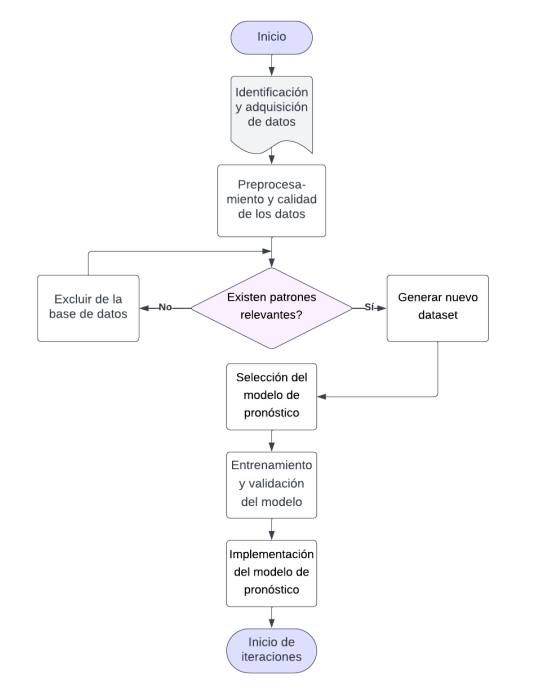
\includegraphics[scale=0.70]{./identificacion de patrones y tendencias.png}
%     \caption{Identificación de patrones y tendencias}
%     \label{fig:identificacion_patrones}
%   \end{center}
% \end{figure}

\section{Preprocesamiento de datos}
En esta sección, se describirán los métodos utilizados para llevar a cabo la
investigación sobre la predicción de compras a partir de un historial de ventas.

\subsection{Obtención de datos}
Los datos usados para generar el modelo fueron proporcionados por la empresa
gastronómica. La misma proporcionó el dataset para ser usado con fines
académicos, los datos presentan las ventas diarias para los diferentes
productos, cuenta con 6 meses de registro desde el 17 de abril del 2023 hasta el
15 de octubre del 2023.

Los datos originales suministrados están conformados por los siguientes
datasets:
\begin{itemize}
  \item productos.csv
  \item ventas.csv
\end{itemize}

Los datos vienen organizados en forma tabular, cada archivo presenta
información separada relacionada con los diferentes productos y el registro de
ventas histórico.

\vspace{1\baselineskip}
\textbf{productos.csv}

Estructura inicial de la tabla de productos (informacion de los 5 primeros
productos(Fig. \ref{fig:priemeros_5productos})).

\begin{figure}[H]
  \begin{center}
    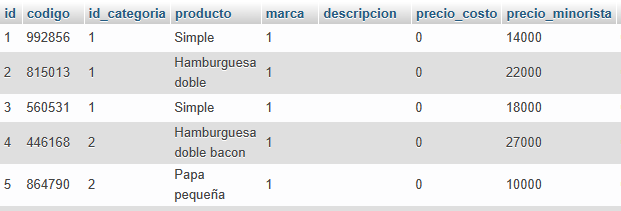
\includegraphics[scale=0.90]{./tabla_producto.png}
    \caption{Estructura inicial de la tabla productos.csv}
    \label{fig:priemeros_5productos}
  \end{center}
\end{figure}

\textbf{ventas.csv}

Estructura inicial de la tabla de ventas(con información de 6 registros (Fig.
\ref{fig:ventas_original})).

\begin{figure}[H]
  \begin{center}
    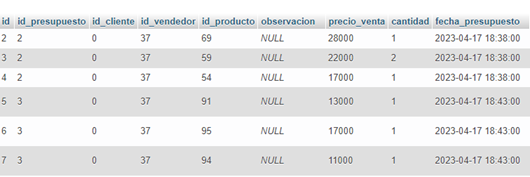
\includegraphics[scale=0.90]{./ventas_tabla.png}
    \caption{Estructura inicial de la tabla  ventas.csv}
    \label{fig:ventas_original}
  \end{center}
\end{figure}

%MODELADO
\subsection{Modelado de datos}
En el siguiente apartado se estara realizando el proceso de limpieza de los
datos para la obtención de los parametros a utilizar.

\vspace{1\baselineskip}

Se obtuvieron las columnas necesarias de la tabla productos para el desarrolo
del proyecto, desde la base de datos MySQL herramienta utilizada para el
almacenamiento de los datos.

\vspace{1\baselineskip}
Hay varios sistemas de gestión de bases de datos gratuitos o de bajo coste disponibles, como MySQL, PostgreSQL o SQLite. Cuando comparas MySQL con otros sistemas de bases de datos, piense en lo que es más importante para usted. Características de rendimiento (como compatibilidad o extensiones de SQL),
soporte, condiciones de licencia y precio, todo son factores a tener en cuenta \cite{dubois2013mysql}.

Dadas estas consideraciones, MySQL tiene muchas cualidades atractivas:

\begin{itemize}
  \item Velocidad.
  \item Facilidad de uso.
  \item Soporte de lenguaje de consulta. MySQL entiende SQL (consulta estructurada
        Language), el lenguaje estándar elegido para todos los sistemas de bases de
        datos modernos.
  \item Capacidad. El servidor MySQL es multihilo, lo que permite que muchos clientes se conecten a él al mismo tiempo. Cada cliente puede usar múltiples bases de datos simultáneamente.
  \item Conectividad y seguridad. MySQL es completamente en red, y las bases de datos se pueden acceder desde cualquier lugar de Internet, lo que le permite compartir sus datos con cualquier persona, en cualquier lugar.
  \item Portabilidad. MySQL se ejecuta en muchas variedades de Unix y Linux, así como en otros sistemas como Windows.
  \item Disponibilidad y costos. MySQL es un proyecto de código abierto disponible bajo múltiples términos de licencia

\end{itemize}



La siguiente consulta SQL selecciona las columnas \texttt{id} y
\texttt{producto} de la tabla \texttt{productos}, donde la columna
\texttt{anulado} tiene un valor nulo:
\begin{center}
  \begin{verbatim}
    SELECT id, producto
    FROM productos
    WHERE anulado IS NULL;
  \end{verbatim}
\end{center}
\begin{figure}[H]
  \begin{center}
    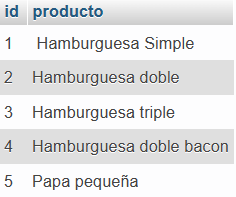
\includegraphics[scale=0.90]{./primeros_5productos.png}
    \caption{Datos de la tabla productos(Los primeros 5 productos)}
    \label{fig:priemeros_5productos}
  \end{center}
\end{figure}

En la tabla \ref{tab:productos} se muestra una descripción de cada una de las
columnas de productos.

\begin{table}[H]

  \begin{tabular}{|c|l|}  % Usamos "l" para alinear a la izquierda
    \hline
    \rowcolor{gray!50} \textbf{Columna} & \textbf{Descripción}                     \\
    \hline
    id                                  & el id del producto (identificador unico) \\
    producto                            & el nombre del producto                   \\
    \hline
  \end{tabular}
  \centering
  \caption{ Descripción de datos de la tabla de productos}
  \label{tab:productos} % Asigna una etiqueta a la tabla
\end{table}

La consulta SQL a continuación selecciona las columnas \texttt{id\_producto},
\texttt{cantidad}, y \texttt{fecha\_venta} de la tabla \texttt{ventas} para las
transacciones que tuvieron lugar en el período desde el 17 de abril de 2023
hasta el 15 de octubre de 2023 donde la columna \texttt{anulado} tiene un valor
nulo (Figura:\ref{fig:fecha_venta}):

\begin{verbatim}
  SELECT id_producto, cantidad, fecha_venta
  FROM ventas
  WHERE fecha_venta BETWEEN '2023-04-17' AND '2023-10-15'
  AND anulado IS NUL;
\end{verbatim}
\begin{figure}[H]
  \begin{center}
    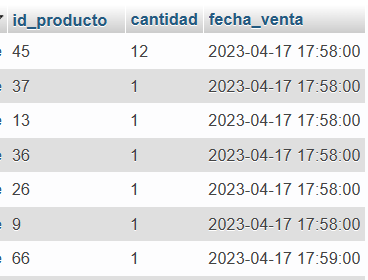
\includegraphics[scale=0.90]{./ventas_fecha.png}
    \caption{Datos de la tabla ventas}
    \label{fig:fecha_venta}
  \end{center}
\end{figure}

En la tabla \ref{tab:ventas_fechas} se muestra una descripción de cada una de
las columnas de productos.

\begin{table}[H]

  \begin{tabular}{|c|l|}  % Usamos "l" para alinear a la izquierda
    \hline
    \rowcolor{gray!50} \textbf{Columna} & \textbf{Descripción}                     \\
    \hline
    id\_producto                        & el id del producto (identificador unico) \\
    catidad                             & cantidad de venta                        \\
    fecha\_venta                        & fecha de la venta                        \\
    \hline
  \end{tabular}
  \centering
  \caption{ Descripción de datos de la tabla ventas}
  \label{tab:ventas_fechas} % Asigna una etiqueta a la tabla
\end{table}

%ESCALADO

\subsection{Escalado de datos}

El escalado de datos es un proceso esencial en el análisis de datos y la estadística que ajusta los valores de las variables para que compartan una misma escala o propiedades específicas.

\vspace{1\baselineskip}
La consulta SQL se enfoca en el escalado de datos de ventas de productos durante un periodo del 17 de abril al 15 de octubre, excluyendo ventas anuladas. La consulta agrupa los resultados por producto y fecha de venta, permitiendo así obtener una visión escalada de la cantidad total vendida de cada producto a lo largo del tiempo, lo que facilita la identificación de tendencias y patrones en las ventas.

\begin{verbatim}
  SELECT id_producto, SUM(cantidad) AS Cantidad, fecha_venta
  FROM ventas
  WHERE fecha_venta BETWEEN '2023-04-17' AND '2023-10-15'
  AND anulado IS NULL
  GROUP BY id_producto, fecha_venta;
\end{verbatim}

\begin{figure}[H]
  \begin{center}
    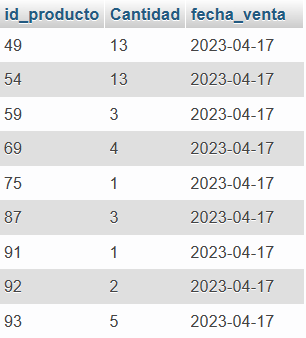
\includegraphics[scale=0.90]{./escalado.png}
    \caption{Datos escalados(muestra de la tabla ventas)}
    \label{fig:escalado}
  \end{center}
\end{figure}

\begin{table}[H]

  \begin{tabular}{|c|l|}  % Usamos "l" para alinear a la izquierda
    \hline
    \rowcolor{gray!50} \textbf{Columna} & \textbf{Descripción}                               \\
    \hline
    id\_producto                        & el id del producto                                 \\
    catidad                             & suma de la cantidad de ventas por fecha y producto \\
    fecha\_venta                        & fecha de la venta                                  \\
    \hline
  \end{tabular}
  \centering
  \caption{ Descripción de datos escalados de la tabla ventas }
  \label{tab:tabla_scalada} % Asigna una etiqueta a la tabla
\end{table}

%ANALISIS DE LOS DATOS
\subsection{Análisis de los datos }
El objetivo principal de esta etapa es explorar y comprender en profundidad los datos, lo que resulta fundamental para una sólida preparación y análisis de los mismos. Esta comprensión más profunda del problema de negocio nos permitirá seleccionar modelos de predicción y tomar decisiones más fundamentadas. Durante el proceso de limpieza y preparación de los datos, se han identificado características relevantes que proporcionarán información valiosa para las fases posteriores del análisis y la toma de decisiones.

\vspace{1\baselineskip}
Como se observa(Figura: \ref{fig:fecha_venta}), la base de datos de entrenamiento es limitada en términos de variables disponibles. En este escenario, se ha seleccionado exclusivamente la fecha como variable de entrada y se ha focalizado en un producto específico, en este caso, la“Hamburguesa simple” con id\_producto 49, debido a su alta demanda. Se han recopilado 182 registros ya agrupados por día, lo que equivale a 182 días de datos. El propósito de este enfoque es analizar el comportamiento de las ventas de dicho
producto en relación al tiempo y buscar patrones que puedan mejorar la precisión del modelo de predicción.

\begin{figure}[H]
  \begin{center}
    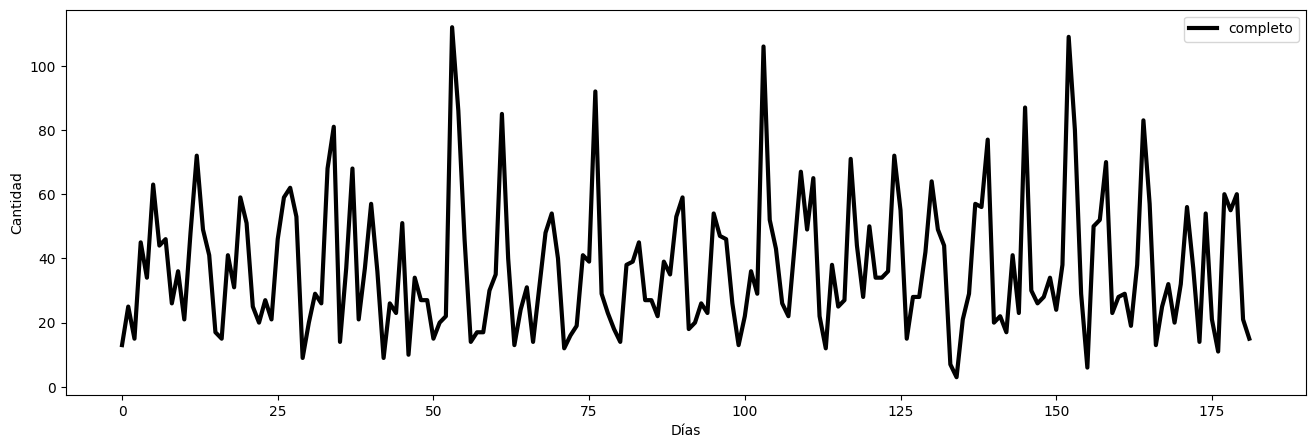
\includegraphics[scale=0.40]{./serie_normal_completa.png}
    \caption{Serie temporal de las ventas totales por día}
    \label{fig:serie_completa}
  \end{center}
\end{figure}

%   En la tabla \ref{tab:ventas} se muestra una descripción de cada una de las columnas de ventas.
%   

% \section{Enfoque}
% El desarrollo de un sistema de compras inteligentes que utiliza un histórico de ventas como fuente principal de información. El objetivo principal es optimizar la gestión de insumos gastronómicos.

% \begin{itemize}
% \item Recopilación y análisis de datos cuantitativos de ventas históricas para desarrollar un modelo predictivo. Esto abarcaría la identificación de patrones de ventas, el uso de algoritmos de aprendizaje automático para predecir futuras compras y la evaluación de la precisión del sistema. 
% \item Aplicación de métricas cuantitativas para evaluar el rendimiento del sistema en términos de eficiencia, impacto en las ventas y beneficios para la entidad objeto de estudio.

% \end{itemize}

% \section{Alcance de la investigación cuantitativa}
% El alcance de esta investigación descriptiva se enfoca en proporcionar una visión detallada y exhaustiva de la aplicación de un sistema inteligente de gestión de compras basado en el histórico de ventas en un local gastronómico ubicado en Ciudad del Este. 
% Se describirá el proceso de recopilación de datos históricos de ventas, incluyendo la fuente de los datos, el periodo de tiempo cubierto y la naturaleza de la información registrada.
% Se proporcionará una descripción completa de cómo opera el sistema inteligente computarizado, incluyendo su arquitectura, algoritmos de pronóstico, y la forma en que utiliza los datos históricos para generar predicciones de demanda.

%VARIABLES DE ENTRADA Y SALIDA
\subsection{Definición de las variables de entrada y salida}

Se han considerado estas variables como variables de entrada debido a que, a través del análisis de la serie temporal de ventas, se han identificado patrones y tendencias significativas que impactan en las ventas del producto.

\vspace{1\baselineskip}
El mes, el día del mes, el día de la semana, la presencia de días festivos y la estación del año influyen directamente en el comportamiento de las ventas. 

\vspace{1\baselineskip}
El promedio de venta mensual varía, lo que indica una estacionalidad en la demanda. Las ventas tienden a aumentar hacia el final e inicio del mes, posiblemente relacionado con el ciclo de pagos de los consumidores. La influencia de los días de la semana sugiere que los fines de semana son momentos clave para las ventas. La presencia de días festivos genera picos en las ventas, lo que puede estar vinculado a la celebración y al aumento de la
demanda en esas fechas. Por último, la estación del año también desencadena cambios en las ventas, con un aumento en verano, lo que respalda la necesidad de considerar esta variable en el modelo para una predicción más precisa.

\vspace{1\baselineskip} Teniendo todas estas informaciones, se procede a la
conversión de estas características en variables de entrada y salida para el
aprendizaje del modelo, y se asegura de que estén representadas en formato
numérico.

\begin{table}[H]
  \begin{tabular}{|c|l|l|}  % Usamos "l" para alinear a la izquierda
    \hline
    \rowcolor{gray!50} \textbf{Columna} & \textbf{Descripción}              & \textbf{Dato numerico} \\
    \hline
    mes                                 & variable mes Rango                & 1-12                   \\
    dia                                 & variable dias del mes Rango       & 1-31                   \\
    dia\_semana                         & variable dia de la semana Rango   & 0-6                    \\
    dia\_festivo                        & variable dia festivo Rango        & 0-1                    \\
    estacion                            & variable estaciones del año Rango & 0-3                    \\
    \hline
  \end{tabular}
  \centering
  \caption{ Variables de entrada}
  \label{tab:variables_de _entrada} % Asigna una etiqueta a la tabla
\end{table}

La siguiente consulta SQL realiza un análisis de ventas de un producto con
id\_producto igual a 49. Agrupa los datos por fecha de venta y calcula diversas
métricas relacionadas con la fecha, como el mes, el día, el día de la semana y
si la fecha es un día festivo. También determina la estación correspondiente a
cada fecha y agrega información sobre la cantidad total de ventas y la suma de
las cantidades vendidas para cada día. En resumen, esta consulta proporciona un
resumen detallado de las ventas del producto 49, organizado por fecha y con
métricas relacionadas con la fecha para su posterior utilización.

\begin{verbatim}
  SELECT MONTH(fecha_venta) AS mes, 
  DAY(fecha_venta) AS dia, 
  DAYOFWEEK(fecha_venta) AS dia_semana, 
  IFNULL((SELECT 1 FROM dias_festivos df 
  WHERE CAST(v.fecha_venta AS date)=df.fecha),0) AS dia_festivo, 
  (SELECT estacion FROM estaciones e 
  WHERE cast(v.fecha_venta AS date) 
  BETWEEN e.fecha_inicio AND e.fecha_fin) AS estacion,
  COUNT(id_venta) AS cantidad_ventas, 
  SUM(v.cantidad) AS cantidad 
  FROM ventas v 
  WHERE id_producto = 49 
  GROUP BY CAST(fecha_venta AS date)
\end{verbatim}

% Tabla (\ref{fig:tabla_resultante})resultante en formato .csv con el exportador
% de MySQL
\begin{figure}[H]
  \begin{center}
    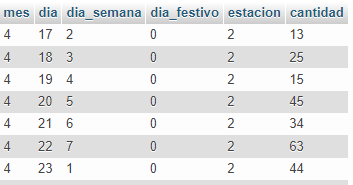
\includegraphics[scale=0.90]{./tabla_resultante.png}
    \caption{Tabla resultante con las variables de entrada}
    \label{fig:tabla_resultante}
  \end{center}
\end{figure}

%LECTURA Y ESCALADO

\subsection{Lectura y escalado del dataset en Python}
% En este trabajo se realiza todo el proceso en el software Python.

% \vspace{1\baselineskip}
La elección de Python como lenguaje de programación se fundamenta en su destacado uso en el campo de la inteligencia artificial, respaldado por una amplia gama de bibliotecas y una comunidad activa\cite{mirjalili2020python}. En cuanto al entorno de pruebas, se ha optado por Google Colab debido a su facilidad de uso y su gratuidad, lo que lo convierte en una opción conveniente para el desarrollo y la prueba de modelos de inteligencia artificial.

\vspace{1\baselineskip}
Los datos se preparan de manera similar tanto para las pruebas en el modelo de regresión lineal como para el modelo LSTM, lo que implica el proceso de escalado y la división en variables de entrada y salida (Figura: \ref{fig:lectura_escalado}).

% En Python, se emplea la biblioteca pandas para la lectura de archivos CSV, y para el escalado, se recurre al MinMaxScaler de la librería sklearn .

\vspace{1\baselineskip}
Python es un lenguaje muy maduro, versátil, y se puede utilizar como una plataforma specífica para el Data Science, gracias a su gran ecosistema de librerías científicas y a su comunidad, que es muy activa \cite{chilet2023elaboracion}.

\vspace{1\baselineskip}
En este proyecto se emplean algunas de ellas que nos facilitaran el proceso a la hora de realizar diferentes
funciones.

\begin{itemize}
  \item \textbf{NumPy:} Ofrece una amplia gama de funciones matemáticas y herramientas para trabajar con datos numéricos, como generadores de números aleatorios, rutinas de álgebra lineal, transformadas de Fourier y más. Esto hace que NumPy sea una biblioteca esencial en aplicaciones científicas y de análisis de datos, ya que proporciona las herramientas necesarias para realizar cálculos numéricos de manera eficiente y rápida \cite{numpy-website}. 
  \item \textbf{Pandas:} Es una biblioteca de Python ampliamente utilizada en la manipulación y análisis de datos. Ofrece un objeto eficiente llamado DataFrame para trabajar con datos tabulares, facilitando la lectura y escritura de datos desde diversas fuentes \cite{pandas-website}. 
  \item \textbf{Matplotlib:} Esta librería de software gráfico permite la generación de gráficos en dos dimensiones, a partir de datos contenidos en listas o arrays. Junto con Pandas han sido las dos librerías de Python que más se han empleado en el proyecto para el tratamiento de los datos \cite{MatplotlibWebsite}.
  \item \textbf{TensorFlow:} Es una potente biblioteca de aprendizaje automático que permite a los desarrolladores y científicos de datos diseñar, entrenar y desplegar modelos de inteligencia artificial en una amplia gama de aplicaciones. \cite{tensorflow-website}.
  \item  \textbf{Keras:} Es una biblioteca de alto nivel para construir y entrenar redes neuronales en Python. Ofrece una interfaz sencilla y modular, siendo valiosa para desarrolladores y científicos de datos. Aunque es compatible con varios backends, TensorFlow se utiliza comúnmente en combinación con Keras para proyectos de aprendizaje profundo \cite{keras-doc}.
  \item \textbf{Scikit-Learn:} Es una librería de aprendizaje automático que contiene herramientas para la predicción de series temporales, incluyendo modelos de regresión y redes neuronales \cite{sepulveda2023analisis}.
\end{itemize}

Además de estas librerías, existen otras herramientas que se pueden utilizar en Python para la predicción de series temporales, como Prophet, que es una librería para el análisis y la predicción de series temporales con estacionalidad.

\begin{figure}[H]
  \begin{center}
    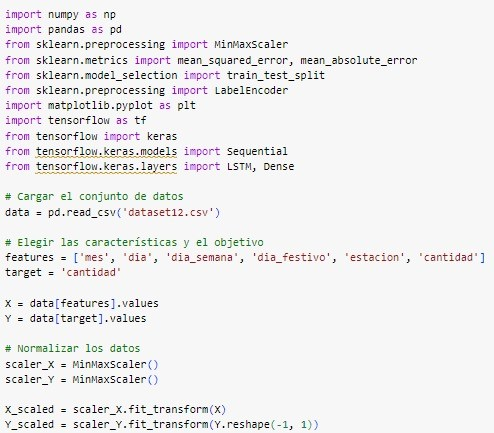
\includegraphics[scale=0.90]{./lectura_escalado.jpg}
    \caption{Codigo de lectura y escalado del dataset en Python}
    \label{fig:lectura_escalado}
  \end{center}
\end{figure}

El gráfico de violín es una herramienta valiosa en el análisis de datos y, en particular, en el contexto de escalado de datos, ya que proporciona una representación más completa y detallada de las distribuciones, lo que puede ayudar a comprender mejor la estructura de los datos y evaluar los efectos del escalado en la distribución de datos.

\vspace{1\baselineskip}
En el grafico \ref{fig:grafico_violin} se puede observar que todas las variables de entrada estan escaladas entre 0 y 1 incluyendo el set train,validación y test.
\begin{figure}[H]
  \begin{center}
    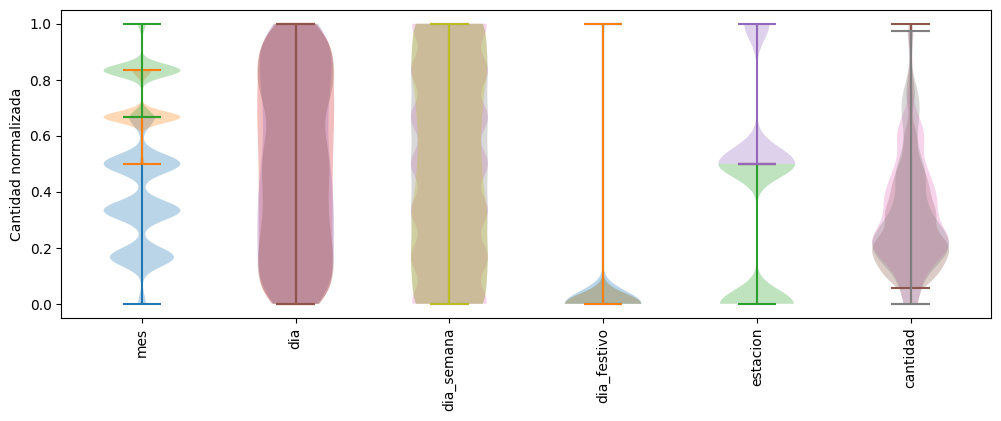
\includegraphics[scale=0.50]{./grafico tipo violin de escalado.png}
    \caption{Grafico en violín incluyendo los tres set train, validación y test}
    \label{fig:grafico_violin}
  \end{center}
\end{figure}

En el grafico \ref{fig:grafico_violin_salida} se puede observar que los datos
de salida también estén escaladas correctamente.
\begin{figure}[H]
  \begin{center}
    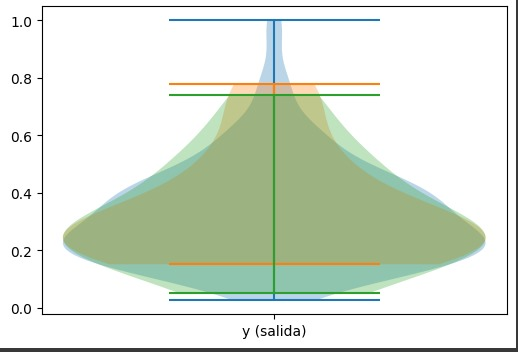
\includegraphics[scale=0.50]{./grafico_violin_salida.jpg}
    \caption{Gráfico en violín de los datos de salida escaladas}
    \label{fig:grafico_violin_salida}
  \end{center}
\end{figure}

%DISTRIBUCION DE LOS DATOS
\subsection{Distribución del conjunto de datos}

En el proceso de entrenamiento, es fundamental dividir el conjunto de datos en
tres conjuntos distintos:

\begin{itemize}
  \item \textbf{Conjunto de Entrenamiento (Train)}: Este conjunto se utiliza para entrenar el modelo, lo que significa que el modelo aprenderá de estos datos durante el proceso de entrenamiento.

  \item \textbf{Conjunto de Validación (Val)}: El conjunto de validación se emplea para evaluar si el modelo está sobreajustando los datos de entrenamiento. Ayuda a ajustar parámetros y prevenir el sobreajuste.

  \item \textbf{Conjunto de Prueba (Test)}: Este conjunto no se utiliza durante el entrenamiento del modelo y contiene datos con valores desconocidos. Se utiliza al final para evaluar la precisión del modelo en un entorno real, ya que no ha tenido acceso a estos datos previamente.
\end{itemize}

Se toma inicialmente 70\% train, 15\% val y 15\% test, como valores comúnmente
utilizados para estos casos.
\begin{figure}[H]
  \begin{center}
    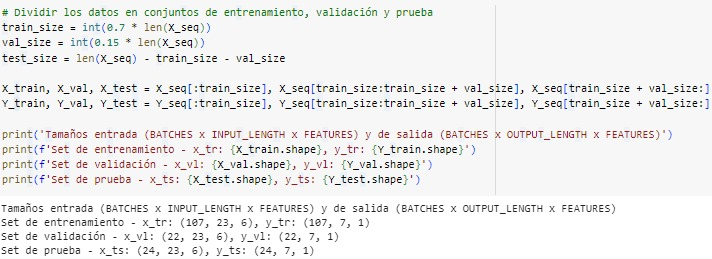
\includegraphics[scale=0.75]{./divisionde _datos.jpg}
    \caption{Codigo de distribución de los datos.}
    \label{fig:distribucion_algoritmo}
  \end{center}
\end{figure}

\begin{figure}[H]
  \begin{center}
    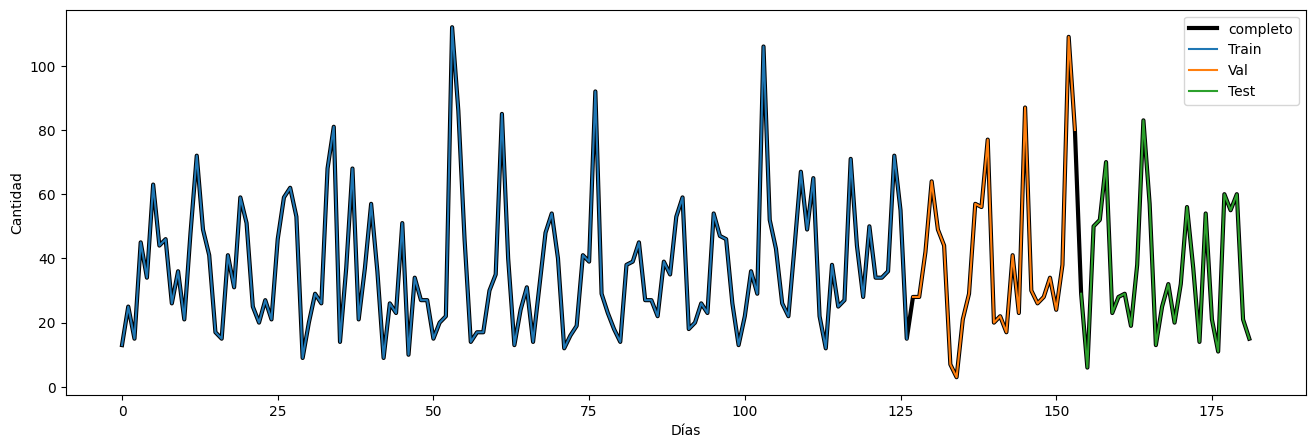
\includegraphics[scale=0.40]{./serie_normal_dividida.png}
    \caption{Distribución de los datos, ventas totales por día.}
    \label{fig:distribucion_datos}
  \end{center}
\end{figure}

%APLICACION Y COMPARACION
\section{Predicción de demanda}

%REGRESION LINEAL
\subsection{Modelo de Regresión lineal}


Para la implementación de regresión lineal, se ha optado por utilizar el
SGDRegressor de la biblioteca sklearn. En lo que respecta a la elección de
hiperparámetros, se han seleccionado valores comunes para un modelo de
regresión lineal implementado a través del algoritmo de Descenso de Gradiente
Estocástico (SGD). Estos hiperparámetros son los siguientes:

\begin{itemize}
  \item \textbf{loss}: Es una función de pérdida en la regresión lineal que mide la diferencia entre las predicciones del modelo y los valores reales. Su objetivo es minimizar esta discrepancia para encontrar la mejor línea de ajuste a los datos.

  \item \textbf{penalty}: Se ha especificado la regularización Ridge, que es una técnica comúnmente utilizada para abordar problemas de regresión. La regularización Ridge ayuda a prevenir el sobreajuste incorporando un término de penalización en la función de pérdida.

  \item \textbf{alpha}: El hiperparámetro de regularización controla la intensidad de la regularización.

  \item \textbf{max\_iter}: Se ha establecido el número máximo de iteraciones permitidas para el descenso de gradiente.

  \item \textbf{tol}: La tolerancia se utiliza para determinar cuándo se ha alcanzado la convergencia.

  \item \textbf{learning\_rate}: Se ha configurado la tasa de aprendizaje como constante a lo largo del proceso de entrenamiento.
\end{itemize}

\textbf{Fase de entrenamiento:}

En esta fase se tiene una cantidad enorme de datos, de la cual se separa una
parte para entrenar al algoritmo y darle toda esta información para que
encuentre los patrones necesarios y después pueda hacer predicciones.

El modelo se entrena con los datos de entrenamiento (X\_train, Y\_train)
utilizando el método .fit(). El modelo ajusta la línea de regresión a estos
datos para realizar predicciones (Figura \ref{fig:estructura_lineal_cap3}).

\vspace{1\baselineskip}
\textbf{Fase de prueba:}

El resto de los datos que quedan, se van a usar para hacer las pruebas. Así le
podemos hacer preguntas al algoritmo y evaluar si las respuestas están bien o
mal, y saber si está aprendiendo o no. Si vemos que no coinciden los datos,
tendremos que agregar más datos o cambiar el método que estamos utilizando.
Pero si se observa que hay entre un 80\% a 90\% de respuestas correctas,
podemos decir que hay un buen grado de aprendizaje y poder utilizar ese
algoritmo.

\vspace{1\baselineskip}
\textbf{Realizar Predicciones en Conjuntos de Datos: (Figura \ref{fig:estructura_lineal_cap3})}

\begin{itemize}
  \item Se realizan predicciones en tres conjuntos de datos diferentes: entrenamiento,
        validación y prueba.
  \item Para cada conjunto, se utiliza el modelo para predecir los valores de la
        variable objetivo.
  \item Las predicciones se almacenan en las variables $Y_{\text{train\_pred}}$,
        $Y_{\text{val\_pred}}$ y $Y_{\text{test\_pred}}$, respectivamente.
  \item Se utiliza el método \texttt{.ravel()} para asegurarse de que las predicciones
        tengan la forma correcta.
\end{itemize}

\begin{figure}[H]
  \begin{center}
    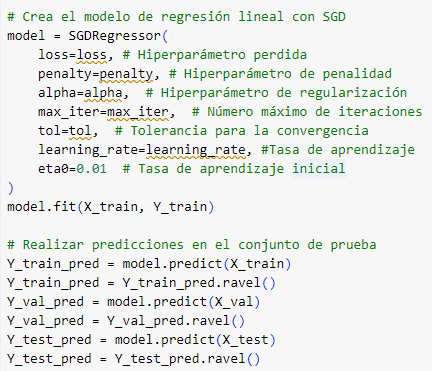
\includegraphics[scale=0.90]{./arquitectura REGRESION LINEAL.png}
    \caption{Codigo de la estructura de regresión lineal.}
    \label{fig:estructura_lineal_cap3}
  \end{center}
\end{figure}

\textbf{Fase de validacion:}

El proceso de validación implica calcular y comparar estas métricas utilizando
los datos de validación y prueba. Un buen modelo de regresión lineal debería
tener valores bajos de MSE y MAE, así como un alto valor de R² en ambos
conjuntos de datos, lo que indica que las predicciones se ajustan bien a los
valores reales. La validación es esencial para evaluar el rendimiento del
modelo en datos no vistos y garantizar su capacidad de generalización.

% \vspace{1\baselineskip}
% \textbf{Matplotlib} es una biblioteca completa para crear visualizaciones estáticas, animadas e interactivas en Python. Matplotlib hace que las cosas fáciles sean fáciles y las difíciles posibles\cite{MatplotlibWebsite}.

\begin{figure}[H]
  \begin{center}
    \includegraphics[scale=0.60]{./Grafico de predicciones con regresión.png}
    \caption{Grafico de lineas con Matplotlib.}
    \label{fig:prediccion_regresion_cap3}
  \end{center}
\end{figure}

%LSTM
\subsection{Modelo LSTM}

La red neuronal LSTM se modela con ayuda de la librería keras, es una librerıa
de codigo abierto de redes neuronales, que se implementa sobre otros frameworks
de aprendizaje automático como Tensorflow, CNTK o theano. Aparecio en 2015 y
fue creada por Fran¸cois Chollet. Tal y como se menciona en su documentación
\cite{keras-doc}, Keras se guía por cuatro principios. Ser amigable para el
usuario, modular, fácilmente extensible e implementada en python.

\vspace{1\baselineskip}
Al configurar una red neuronal LSTM, es común considerar varios hiperparámetros
clave (Codigo \ref{fig:desenpeño}):

\begin{itemize}
  \item \textbf{Unidades de LSTM:} Por lo general, se comienza con un número moderado de unidades en las capas LSTM, como 64 o 128. Aumentar el número de unidades puede ayudar a capturar patrones más complejos, aunque conlleva un mayor riesgo de sobreajuste.

  \item \textbf{Número de capas LSTM:} Para problemas más complejos, es posible agregar capas adicionales. Las arquitecturas con dos capas LSTM son comunes y funcionan bien en muchas aplicaciones.

  \item \textbf{Función de Activación:} Para las capas LSTM, la función de activación predeterminada suele ser “tanh”. No obstante, se pueden explorar otras funciones como “relu” o “sigmoid” según las necesidades del problema.

  \item \textbf{Función de Pérdida:} En problemas de regresión, es común utilizar el "mean squared error" (MSE) como función de pérdida. No obstante, la elección puede variar según el problema en particular.

  \item \textbf{Optimizador:} El “Adam” es un optimizador sólido y ampliamente utilizado en problemas de aprendizaje profundo. Aunque existen otras opciones como “RMSprop,” la elección depende en gran medida del contexto.

  \item \textbf{Tasa de Aprendizaje:} La tasa de aprendizaje es un hiperparámetro crucial. Por lo general, se comienza con un valor bajo, como 0.001, y se ajusta según la convergencia del modelo.

  \item \textbf{Dropout:} La técnica de dropout, aplicada en un porcentaje determinado de neuronas durante el entrenamiento, puede ayudar a prevenir el sobreajuste. Se recomienda iniciar con un valor del 20\% y ajustar según las necesidades del problema.
\end{itemize}

Es importante tener en cuenta que la elección de estos hiperparámetros puede
depender en gran medida del problema específico y requiere experimentación para
encontrar la configuración óptima.

\vspace{1\baselineskip}
\textbf{Diseño y Entrenamiento del Modelo LSTM:}
\begin{itemize}
  \item Diseña un modelo LSTM.
  \item Compila el modelo con función de pérdida y optimizador.
  \item Entrena el modelo con datos de entrenamiento.
\end{itemize}

\begin{figure}[H]
  \begin{center}
    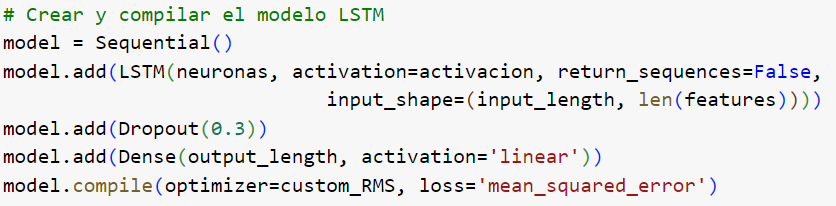
\includegraphics[scale=0.60]{./arquitectura LSTM.png}
    \caption{Codigo de la estructura del LSTM.}
    \label{fig:estructura_lstm}
  \end{center}
\end{figure}

\textbf{Validación del Modelo:}

\vspace{1\baselineskip}

Evalúa el rendimiento del modelo con datos de prueba.

\vspace{1\baselineskip}

\textbf{Conjunto de prueba 1:}
\begin{itemize}
  \item División del conjunto de datos: 70\% train, 20\% validation, 10\% test
  \item Optimizador: Adam
  \item Pérdida: Mean Squared Error (mean\_squared\_error)
  \item Épocas: 200
  \item Tamaño de lotes: 30
  \item Estructura de red: 1 capa oculta con 64 neuronas
  \item Función de activación: Linear
\end{itemize}

\vspace{1\baselineskip}

\begin{figure}[H]
  \begin{center}
    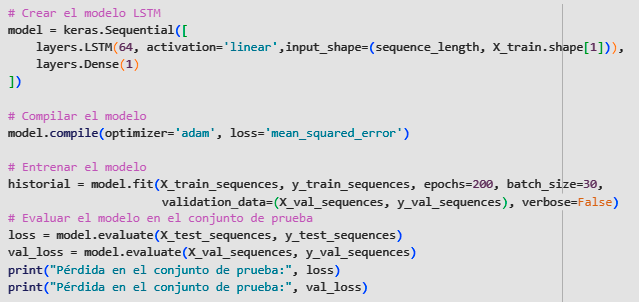
\includegraphics[scale=0.80]{./arqui1ie.png}
    \caption{Codigo de la estructura del LSTM datos de prueba 1.}
    \label{fig:arqui1ie}
  \end{center}
\end{figure}

El código presentado (Figura \ref{fig:arqui1ie}) es un ejemplo de construcción,
entrenamiento y evaluación de un modelo de red neuronal recurrente LSTM para un
problema de regresión. Se inicia con la definición del modelo, que consta de
una capa LSTM y una capa densa, seguido de la compilación con el optimizador
Adam y la métrica de pérdida de error cuadrático medio. El modelo se entrena
durante 200 épocas con lotes de tamaño 30, utilizando datos de entrenamiento y
validación. Luego se evalúa en un conjunto de prueba independiente y se calcula
la pérdida en el conjunto de validación para supervisar el rendimiento del
modelo. Las pérdidas resultantes se imprimen como indicadores de la calidad de
las predicciones del modelo en diferentes conjuntos de datos.

\begin{figure}[H]
  \begin{center}
    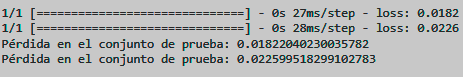
\includegraphics[scale=0.80]{./res1i.png}
    \caption{Rendimiento de datos de prueba 1.}
    \label{fig:rend1}
  \end{center}
\end{figure}

\textbf{27ms/step y 28ms/step:} Estas cifras (Figura \ref{fig:rend1}) indican el tiempo promedio que le toma al modelo procesar una iteración o paso de entrenamiento (epoch). En este caso, el modelo tarda aproximadamente 27-28 milisegundos en completar cada paso de entrenamiento. Este valor es útil para evaluar la eficiencia computacional del entrenamiento del modelo.

\vspace{1\baselineskip}
\textbf{loss: 0.0182 y loss: 0.0226:} Estos valores de la (Figura \ref{fig:rend1}) representan la pérdida (loss) del modelo en los datos de entrenamiento en dos momentos diferentes del entrenamiento. La pérdida es una medida que indica cuán diferente son las predicciones del modelo de los valores reales en los datos de entrenamiento. En este contexto, una pérdida de 0.0182 y 0.0226 sugiere que el modelo está haciendo buenas predicciones en los datos de entrenamiento, con 0.0182 siendo un valor ligeramente mejor (menos pérdida) que 0.0226. Sin embargo, es importante recordar que estos valores solo representan el rendimiento del modelo en los datos de entrenamiento y no necesariamente reflejan su capacidad para generalizar en datos no vistos, como el conjunto de prueba.

\begin{figure}[H]
  \begin{center}
    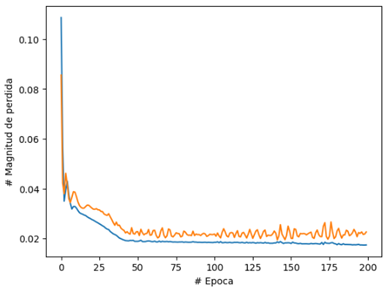
\includegraphics[scale=0.80]{./imagenlstm1.png}
    \caption{Grafico de predicción LSTM prueba 1}
    \label{fig:res2}
  \end{center}
\end{figure}

\vspace{1\baselineskip}
\textbf{Conjunto de prueba 2:}
\begin{itemize}
  \item División del conjunto de datos: 70\% train, 15\% validation, 15\% test
  \item Optimizador: Adam (learning\_rate=0.001)
  \item Pérdida: mean\_squared\_error
  \item Épocas: [50, 100, 200]
  \item Tamaño de lotes: [5, 10, 15]
  \item Estructura de red: 1 capa oculta con [32, 64, 128] neuronas
  \item Función de activación: relu
\end{itemize}

\begin{figure}[H]
  \begin{center}
    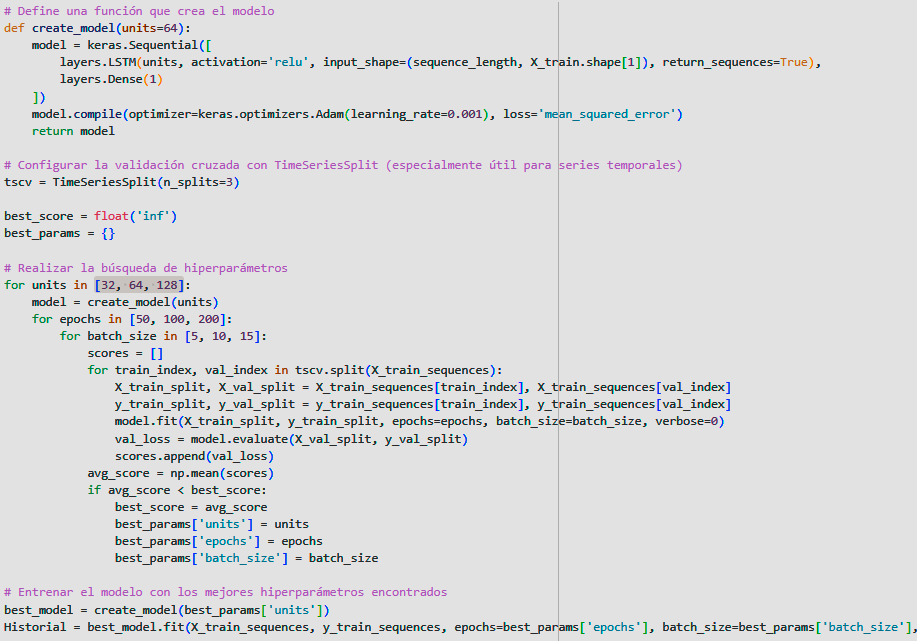
\includegraphics[scale=0.50]{./arqui2i.png}
    \caption{Codigo de la estructura del LSTM datos de prueba 2.}
    \label{fig:arqui2i}
  \end{center}
\end{figure}

El código (Figura \ref{fig:arqui2i}) presenta un proceso de búsqueda de
hiperparámetros para un modelo LSTM en datos de series temporales. Se definen
diferentes configuraciones de modelos con variaciones en el número de unidades
LSTM, épocas de entrenamiento y tamaño de lote.

\vspace{1\baselineskip}
Estos modelos se evalúan en un esquema de validación cruzada específico para series temporales, y se promedian las puntuaciones de rendimiento en las
divisiones de validación.

\vspace{1\baselineskip}
Los valores de hiperparámetros que generan la mejor puntuación se almacenan en best\_params.

\vspace{1\baselineskip}
Luego, se crea un modelo con estos hiperparámetros óptimos y se entrena en todo el conjunto de datos de entrenamiento.

\vspace{1\baselineskip}
Esta metodología busca encontrar la configuración de modelo que se ajuste mejor a los datos de series temporales, garantizando que el modelo sea robusto y pueda generalizar efectivamente a datos futuros.

\begin{figure}[H]
  \begin{center}
    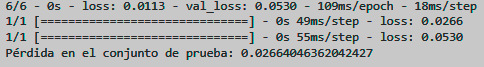
\includegraphics[scale=0.80]{./res2i.png}
    \caption{Rendimiento de datos de prueba 2.}
    \label{fig:res2}
  \end{center}
\end{figure}

En el contexto de un modelo LSTM entrenado en series temporales, los valores proporcionados representan métricas clave para evaluar su desempeño (Figura \ref{fig:res2}). 6/6 indica que se han completado seis épocas de entrenamiento,
mientras que 0s no especifica el tiempo transcurrido. La perdida (loss) de 0.0113 en el conjunto de entrenamiento señala un buen ajuste del modelo a los datos de entrenamiento, mientras que la val\_loss de 0.0530 en el conjunto de validación es ligeramente más alta, lo que sugiere que el modelo podría tener dificultades
para generalizar. Los tiempos en milisegundos por época y por paso (109ms/epoch y 18ms/step) reflejan la eficiencia de entrenamiento del modelo. En resumen, estas métricas ofrecen información sobre la capacidad del modelo para aprender
de los datos de entrenamiento y su habilidad para generalizar efectivamente a datos no vistos en el conjunto de validación, lo que es crucial en aplicaciones de series temporales.

\begin{figure}[H]
  \begin{center}
    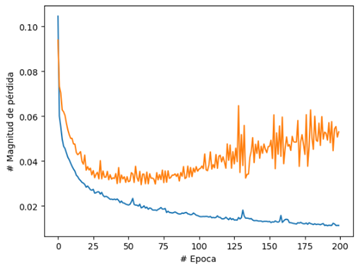
\includegraphics[scale=0.80]{./Imagenlstm2.png}
    \caption{Grafico de predicción LSTM prueba 2}
    \label{fig:res2}
  \end{center}
\end{figure}

\section{Prototipo del sistema}

El sistema web se desarrollará utilizando una combinación de tecnologías, que incluye PHP para la lógica del servidor, JavaScript para la interactividad y dinamismo en el lado del cliente, y HTML y CSS para la estructura y el diseño de la interfaz \cite{nixon2014learning}. Esta elección de tecnologías permite la creación de una aplicación web versátil y receptiva, que ofrece una experiencia de usuario intuitiva y eficiente, al tiempo que garantiza un sólido procesamiento en el servidor para gestionar las diversas funcionalidades del sistema.

\vspace{1\baselineskip}
El nuevo modelo debe garantizar el abastecimiento oportuno de productos sin
incurrir en sobre stock, minimizando el costo de inventario y facilitando el trabajo del área de compras. Para esto se propone diseñar y codificar una aplicación web que realice estas actividades, sin que los analistas deban realizar cálculo matemáticos complejos.


\vspace{1\baselineskip}
\textbf{Levantamiento de requisitos}

Importancia de la selección de una buena técnica de levantamiento de requerimientos 
Una técnica, es una serie de pasos documentados que van de la mano con unas reglas para su uso y criterios para verificar su corrección. Una técnica usualmente aplica a un proceso en el
modelo de procesos. Algunas veces, dicha técnica incluye una notación y/o una herramienta asociada \cite{mejia2009tecnicas}.

\vspace{1\baselineskip}
\textbf{Requisitos del sistema}
 \begin{itemize}

  \item Gestión de productos: 
  
  El sistema debe permitir la creación, modificación y eliminación de productos, incluyendo detalles como nombre.

  \item Órdenes de compra: 
  
  El sistema debe permitir la creación de órdenes de compra, especificando los productos y las cantidades.

  \item Órdenes de venta:
  
  Debe ofrecer la capacidad de crear órdenes de venta para registrar las transacciones, especificando los productos, las cantidades.
  
  \item Generación de informe: 
  
  Capaz de generar informes sobre las predicciones de los productos.
  
 \end{itemize}

 En el contexto de esta tesis, las entrevistas se utilizaron como una técnica esencial para la recolección de datos y la comprensión de los requerimientos del sistema.

 \vspace{1\baselineskip}
 Las órdenes de compra son vitales para registrar las adquisiciones de insumos, ya que nos permiten especificar los productos y sus cantidades. Asimismo, las órdenes de venta son esenciales para el registro de las ventas de productos finales, lo que proporciona un seguimiento preciso de las transacciones.

 \vspace{1\baselineskip}
La generación de informes cobra importancia para analizar y predecir el comportamiento de los productos, permitiéndonos realizar ajustes necesarios en nuestras predicciones. En resumen, estos requisitos se originaron directamente de la necesidad de abordar eficazmente la problemática de la gestión de insumos gastronómicos y garantizar un funcionamiento óptimo del sistema.
 
\vspace{1\baselineskip}
 El anexo de la tesis se convierte en un recurso valioso para aquellos lectores interesados en explorar en profundidad tanto la investigación cualitativa realizada a través de la entrevista como los aspectos técnicos y prácticos del prototipo desarrollado. Proporciona una visión completa de los dos componentes críticos de este trabajo: la obtención de requerimientos a través de entrevistas y la implementación técnica del sistema prototipo.

 
% \begin{figure}[H]
%   \begin{center}
%     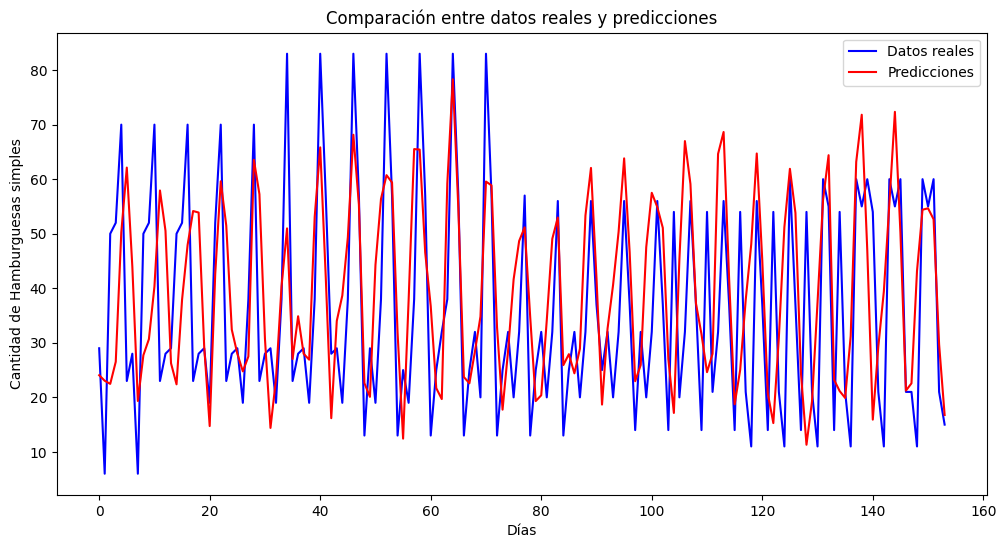
\includegraphics[scale=0.50]{./predicción 7 días.png}
%     \caption{Grafico de predicción con LSTM.}
%     \label{fig:grafico_lstm}
%   \end{center}
% \end{figure}

% Los tres valores muestran una proximidad aceptable, lo que indica que el modelo
% tiene una capacidad de generalización satisfactoria (Figura
% \ref{fig:desenpeño}).
% \begin{figure}[H]
%   \begin{center}
%     \includegraphics[scale=0.50]{./comparativo desempeños LSTM.png}
%     \caption{Comparativo de desempeños LSTM.}
%     \label{fig:desenpeño}
%   \end{center}
% \end{figure}

% En este trabajo para evaluar el rendimiento de una red neuronal LSTM se hace
% uso de la gráfica de pérdidas loss. Esta permite evaluar cómo es su evolución
% de los datos en un modelo. Según la literatura entre más grandes las pérdidas
% las predicciones van a estar alejadas del valor real. En la (Figura
% \ref{fig:perdida}) se puede observar la evolución de pérdidas a través de las
% épocas, se evidencia dos señales que corresponden a entrenamiento y validación
% marcados con los colores azul y naranja respectivamente, se infiere que los
% valores decrecen con una alta tasa hasta la época 5 aproximadamente y luego no
% presentan cambios significativos. Las pérdidas son de 0.020 y 0.039 para
% entrenamiento y test respectivamente.

% \begin{figure}[H]
%   \begin{center}
%     \includegraphics[scale=0.50]{./grafico de perdida en las épocas.png}
%     \caption{Grafico de perdida(loss) en las épocas LSTM .}
%     \label{fig:perdida}
%   \end{center}
% \end{figure}

% \section{Afinación de hiperparámetros con base en porcentaje de pérdida RMS}

% \section{Analítica descriptiva}

% \section{Conjunto de datos}

% Cuenta con 3.840 registros de ventas que agrupados por fecha dan un total de 185 registros, que corresponden a la cantidad de ventas diarias del prodcuto mensionado organizados por fechas desde el 17 de abril de 2023 hasta el 15 de octubre de 2023. 

% Se  empleó  un  conjunto  de  datos  recopilados  a  partir  del  número  diario  de  productos vendidos,  obtenido  de la empresa gastronomica que proveyo los datos para el analisis y predicción de la misma, es importante destacar que el conjunto de datos es continuamente actualizado, sin embargo, para los propósitos de esta investigación, se consideró un conjunto de datos con 180 registros que cubren el período desde 17 de Abril del 2023 hasta 15 de Octubre del 2023 de un producto en especifico “hamburgesa simple”.

% Como el objetivo de este proyecto consiste en predecir las ventas del dia, se realiza una gráfica \ref{fig:serie_completa}, la cual nos permite ver la serie temporal de las ventas del producto mencionado. 

% Posteriormente, se dividió el conjunto de datos en tres grupos: entrenamiento, validación y prueba. El grupo de entrenamiento comprendió 148 registros que cubren desde 17 de abril hasta el 9 de septiembre. El grupo de validación incluyó 18 registros, desde 10 de septiembre hasta el 29 de septiembre  y el conjunto de prueba 19 registros desde el 30 de septiembre hasta 18 de octubre.

% \textbf{Lista de requisitos:}

% \begin{itemize}
% % \item Registro de usuarios(Alta, Baja, Modificaciones).
% \item Registro de productos (Alta, Baja, Modificaciones).
% \item Registro de insumos(materia prima) (Alta, Baja,Modificaciones). 
% \item Registro de pedidos/ventas (Alta, Baja, Modificaciones).
% \item Generación de Informes Personalizados: Debe permitir la creación de informes personalizados que muestren datos específicos para análisis.
% \item Análisis de Tendencias: Debe ser capaz de identificar tendencias y patrones en las ventas de insumos, lo que facilita la toma de decisiones basadas en datos.

% \end{itemize}
% \begin{figure}[H]
%     \begin{center}
%       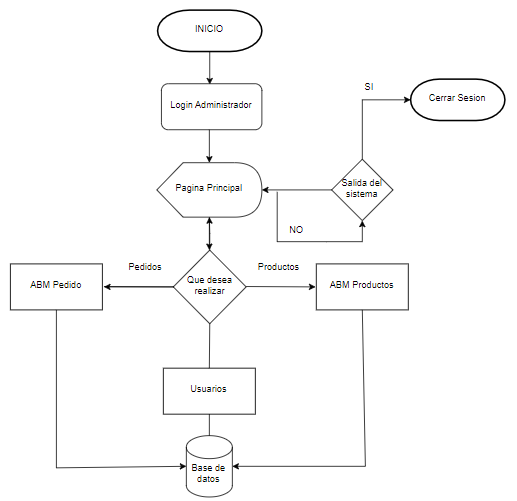
\includegraphics[scale=0.90]{./diseño_procedural.png}
%       \caption{Diseño procedural.}
%       \label{fig:diseño_procedural}
%     \end{center}
%   \end{figure}

% \section{Librerias de uso común en Mching Learning}
% A continuación se instalara y actualizaran las principales librerias mas utilizadas cuando se realizan programas de inteligencia artificial.

% \begin{itemize}
%   \item \textbf{TensorFlow:} Es una plataforma de código abierto de un extremo a otro para el aprendizaje automático. Tiene un ecosistema integral y flexible de herramientas, bibliotecas y recursos comunitarios que permite a los investigadores impulsar lo último en ML y a los desarrolladores crear e implementar fácilmente aplicaciones basadas en ML.
%   Es ampliamente utilizada para desarrollar y entrenar modelos de redes neuronales, incluyendo modelos LSTM (Long Short-Term Memory).
%   \item \textbf{Keras:} Es una interfaz de alto nivel para TensorFlow que facilita la construcción, entrenamiento y evaluación de modelos de redes neuronales, incluyendo modelos LSTM.
% \end{itemize}

% La función de activación utilizada para modelar la no linealidad suele ser la Unidad Lineal Rectificada (ReLU), que puede calcularse más rápido que las funciones tangentes sigmoideas o hiperbólicas utilizadas tradicionalmente y también ofrece interesantes propiedades de convergencia.

% \subsection{Alcance exploratorio.}
% La medida de este alcance abarca la exploración de problemas generalmente poco conocidos, a veces difíciles de conocer.

% \subsection{Alcance descriptivo.}
% La medida de este alcance abarca la descripción del fenómeno, situación, contexto o evento; detalla cómo es y cómo se manifiesta. Busca especificar propiedades, características y rasgos importantes. Describe tendencias de un grupo o población. Es útil para mostrar con precisión los ángulos o dimensiones de un fenómeno, suceso, comunidad, contexto o situación.

% \subsection{Alcance correlacional.}
% La profundidad de este alcance busca establecer relaciones entre variables sin precisar sentido de causalidad, es decir, no analiza relación causal.

% Un ejemplo de este alcance es una investigación que busca averiguar cómo se relacionan las calificaciones de los alumnos de un grado, en las asignaturas: Castellano y Matemática.

% \subsection{Alcance explicativo.}
% La profundidad de este alcance busca establecer relaciones entre variables precisando sentido de causalidad, es decir, analiza relación entre causa y efecto entre variables.

% Un ejemplo de este alcance es una investigación que busca averiguar la relación entre urbanización y alfabetismo en un país, para ver qué variables macrosociales definen el grado de alfabetización de la población del país.

% \section{Diseño}
% Es el plan o estrategia que se desarrolla para obtener la información que se requiere en una investigación, generalmente para verificar la hipótesis. La precisión, amplitud y profundidad de la información obtenida varía en función del diseño elegido \cite{sampieri}.

% En la literatura sobre investigación cuantitativa es posible encontrar diferentes clasificaciones de los diseños; los autores \cite{sampieri} adoptan la siguiente clasificaciòn: investigación experimental e investigación no experimental. A su vez, la primera puede dividirse de acuerdo con las clásicas categorías de Campbell y Stanley (1966) en: preexperimentos, experimentos ``puros'' y cuasiexperimentos. La investigación no experimental, siempre de acuerdo con \cite{sampieri}, se subdivide en diseños transversales y diseños longitudinales.

\vspace{.5 cm}

% \textbf{Ejemplo de diseño en una investigación tecnológica formativa.}

% Aún más que en la investigación en ciencias básicas, es en la investigación tecnológica donde se puede apreciar la importancia del diseño para obtener un buen producto o servicio. Cabe entonces ilustrarlo con un ejemplo tomado dentro de esta última forma de investigación desde la referencia \cite{lan}.

\vspace{.5 cm}

% \textbf{\emph{Metodología para implementar red de área local. (\gls{lan}\@)}}\footnote{Por brevedad, solo se desarrolla la etapa de diseño.}

% Hoy en día, como nunca antes, el ser social necesita estar informado. Para estudiar problemas y tomas de decisiones es necesario disponer de datos precisos, en el lugar y en el instante preciso. En gran medida se logra lo anterior con las redes de computadoras, cuyo objetivo fundamental es compartir recursos e información pues ofrecen acceso a servicios universales de datos tales como: bases de datos, correo electrónico, transmisión de archivos y boletines electrónicos; eliminando el desplazamiento de los individuos en la búsqueda de información y aumentando la capacidad de almacenamiento disponible por cada usuario en un momento determinado.

% Un gran porcentaje de las redes de computadoras se usan para la transmisión de información científica siendo una vía rápida y económica de divulgar resultados y de discutir con otros especialistas afines sobre un tema en cuestión. En este trabajo en particular se aborda la metodología a seguir para la implementación de redes de computadoras de área local; las cuales cumplen todos los objetivos planteados a una escala reducida ya que son propiedad de una sola organización (un solo centro administrativo o fabril) abarcando zonas geográficas de algunos kilómetros como máximo. La experiencia en el campo de \glspl{lan} en el ámbito universitario, donde las mismas se emplean para la gestión administrativa y económica, para la transmisión de información científica y para la enseñanza; ha dejado claro que el diseño, la instalación y puesta a punto de una \gls{wan} suele ser un proceso cuidadoso del cual depende en grado sumo que se cumplan los objetivos para los que se invirtió en dicha red.

% Para su comprensión el trabajo se divide en cinco partes o etapas:
% \begin{itemize}
% \item Etapa de estudio,
% \item Etapa de diseño.\footnote{Solo se desarrolla esta etapa.}
% \item Etapa de elaboración de la solicitud de oferta y selección del vendedor,
% \item Etapa de instalación y puesta en funcionamiento,
% \item Etapa de análisis de las prestaciones y evaluación de los resultados.
% \end{itemize}

% Una vez concluida la primera etapa y aprobado el presupuesto de la red es necesario realizar la etapa del \textit{diseño} de la \gls{lan} para lo cual se deben seguir los siguientes pasos:

\renewcommand{\labelitemi}{$-$}

% \begin{itemize}
% \item Seleccionar la(s) topología(s) y norma(s) de red a emplear,
% \item Seleccionar el soporte de transmisión a utilizar,
% \item Analizar la necesidad de emplear técnicas de conectividad,
% \item Considerar ampliaciones futuras de la red,
% \item Realizar una evaluación primaria del tráfico,
% \item Contemplar las necesidades del personal involucrado en la red,
% \item Modificar, de ser necesario, el flujo de la información y seleccionar el software de aplicación.
% \end{itemize}

% \textit{Seleccionar la topología.} Este paso, el cual es dependiente de los resultados del anterior. Las tres topologías más empleadas son: bus, estrella y anillo; mientras que las normas más comunes son: Ethernet, Token Ring y ArcNet. La selección de los aspectos anteriores trae aparejado escoger la velocidad de transmisión, la distancia máxima a emplear, el método de control de acceso al medio, etc. La elección se realiza a partir de la necesidad particular y de un amplio conocimiento de las topologías y normas existentes. 

% \textit{Seleccionar el Soporte de Transmisión.} Esto está muy relacionado con la norma a emplear y con las características de los puntos a conectar. Es vital realizar una selección adecuada pues una opción equivocada comprometería la eficacia y la velocidad de la transferencia de datos. Para la elección de uno u otro medio de transmisión se debe tomar entre otras cosas las dimensiones de la instalación, el costo, la evolución tecnológica estimada, la facilidad de instalación y el grado de hostilidad electromagnética presente en el entorno. 

% Aunque el \gls{sored}  (del inglés NOS: Netware Operating System) NetWare predomina en el mundo, éste no es siempre la elección adecuada, debido a sus costos y características. En el mercado existen otros \glspl{sored} tales como: LAN Manager, LANServer, LANtastic, Vines, LINUX, Windows NT Server, Windows 2000 Server, etc.; los cuales poseen una determinada cuota de mercado. Para seleccionar el SOR adecuado se debe tener en cuenta:

% \begin{itemize}
% \item El nivel de confidencialidad que brinda a los datos,
% \item Si es del tipo cliente-servidor o de igual a igual,
% \item Grado de tolerancia a fallos que posee,
% \item Memoria RAM necesaria en el servidor y en las estaciones de trabajo,
% \item Facilidades de administración y diagnóstico que brinda,
% \item Si posee o no sistema de correo electrónico,
% \item Características de manipulación de colas de impresión.
% \end{itemize}

% \textit{Analizar la necesidad de emplear técnicas de conectividad.} Esto estará en función de las dimensiones de la organización, del tráfico a cursar y el tipo de equipamiento a interconectar entre otros aspectos. Es necesario conocer en profundidad dichas técnicas para realizar una adecuada selección entre repetidores, puentes, ruteadores, compuertas, servidores de acceso, etc. y lograr su correcta ubicación. La mejor solución muchas veces hace uso de más de un tipo de dispositivo de interconexión.

% \textit{Considerar ampliaciones futuras de la red.} Aún cuando de forma inmediata no sea necesario extender la red ni conectarse a otros, ésta debe poseer la base para que a partir de ella, y en cualquier momento sea posible una ampliación o llegar a formar parte de otras redes.

% \textit{Realizar una evaluación primaria del tráfico.} Aquí debe estimarse el tráfico que circulará en la red y analizar si el mismo no afecta el tiempo de acceso a la información ya otros recursos compartidos. Es importante que una vez instalada y puesta en funcionamiento la \gls{lan} se efectúen periódicamente estudios de este tipo.

% \textit{Contemplar las necesidades del personal involucrado en la red.} Esto es muy importante pues en última instancia éste será el personal que utilizará la red y por lo tanto deben quedar satisfechas sus necesidades de forma tal que la nueva red sea un elemento que facilite su trabajo.

% \textit{Modificar de ser necesario el flujo de información y seleccionar el software de aplicación.} Esto implica la modificación, como última opción, de la manera en que la información circula dentro de la organización y la definición del software de aplicación necesario, ya sea comercial o aquél que se encargará al personal especializado; que conozca las particularidades de la programación en ambiente multiusuario. El software encargado o adquirido debe ser de fácil instalación y aprendizaje. Además se debe velar porque sea posible tener acceso a posteriores actualizaciones y que éstas no sean caras.

% \section{Lenguajes de programación}

% \subsection{Python}
% Python es un lenguaje de programación potente y elegante
% que sea fácil de leer y de entender\cite{python2021python}.

% Tiene estructuras de datos de alto nivel eficientes y un simple pero efectivo sistema de programación orientado a objetos. La elegante sintaxis de Python y su tipado dinámico, junto a su naturaleza interpretada lo convierten en un lenguaje ideal para scripting y desarrollo rápido de aplicaciones en muchas áreas, para la mayoría de plataformas.

% Python se destaca en el ámbito de la inteligencia artificial debido a su capacidad para gestionar conjuntos de datos voluminosos y su facilidad de programación. Su sintaxis concisa y legible lo convierte en una elección ideal para crear prototipos de forma rápida, dinámica y comprensible.
% Además de su amplia popularidad, la razón principal para adentrarse en Python en el contexto del aprendizaje automático es, indiscutiblemente, su vasto ecosistema de recursos previamente desarrollados. 

% \paragraph{Pandas:}
% Es una biblioteca de código abierto que proporciona estructuras de datos flexibles y herramientas de análisis de datos para Python. Su principal estructura de datos es el DataFrame, que permite organizar datos en tablas bidimensionales. Pandas es ampliamente utilizado para la limpieza, manipulación y análisis de datos tabulares, lo que lo hace esencial en el análisis de datos.

% \paragraph{NumPy:}
% Es una biblioteca fundamental para el cálculo numérico en Python. Proporciona soporte para arreglos multidimensionales (llamados ndarrays) y una amplia gama de funciones matemáticas para operaciones en estos arreglos. NumPy es crucial para realizar cálculos numéricos eficientes y es la base de muchas otras bibliotecas de análisis de datos en Python.

% \paragraph{Matplotlib:}
% Es una biblioteca de visualización que permite crear gráficos estáticos de alta calidad. Proporciona una variedad de tipos de gráficos, desde gráficos de líneas y barras hasta histogramas y gráficos de dispersión. Matplotlib es ampliamente utilizado para visualizar datos y resultados en el análisis de datos.

% \paragraph{Seaborn:}
% Es una biblioteca de visualización basada en Matplotlib que simplifica la creación de gráficos estadísticos atractivos. Ofrece una interfaz de alto nivel para crear fácilmente visualizaciones complejas y atractivas, lo que la hace útil para el análisis exploratorio de datos y la presentación de resultados.

% \paragraph{Scikit-learn:}
% Es una biblioteca de aprendizaje automático que proporciona herramientas para tareas comunes de aprendizaje automático, como clasificación, regresión, clustering y selección de modelos. También incluye utilidades para la evaluación de modelos y el preprocesamiento de datos, lo que la convierte en una biblioteca esencial para el análisis de datos relacionados con el aprendizaje automático.

% \paragraph{StatsModels:}
% Es una biblioteca que se utiliza para realizar análisis estadísticos y modelado en Python. Está especialmente orientada a tareas como la regresión lineal y logística, análisis de series temporales y pruebas estadísticas. Es útil para realizar análisis estadísticos rigurosos en el contexto del análisis de datos.

% \paragraph{SciPy:}
% Es una extensión de NumPy que proporciona funcionalidades adicionales para cálculos científicos y técnicos. Incluye módulos para optimización, interpolación, integración numérica, álgebra lineal, transformadas y más. Es una biblioteca esencial para aplicaciones científicas y de ingeniería que involucran cálculos numéricos.

% \paragraph{Plotly:}
% Es una biblioteca que permite crear gráficos interactivos y visualizaciones web en Python. Es útil para crear visualizaciones interactivas para el análisis exploratorio de datos y la presentación de resultados en aplicaciones web.

% \paragraph{Bokeh:}
% Es otra biblioteca para crear gráficos interactivos y aplicaciones web basadas en datos. Ofrece una amplia gama de herramientas para crear visualizaciones interactivas y es especialmente útil para proyectos que requieren interfaces de usuario interactivas.

% \paragraph{Dask:}
% Es una biblioteca que se utiliza para el procesamiento paralelo y distribuido de datos en Python. Permite trabajar con conjuntos de datos grandes y realizar operaciones complejas de manera eficiente en clústeres de computadoras.

% \paragraph{TensorFlow y PyTorch:}
% Si bien estas bibliotecas son conocidas principalmente por el aprendizaje profundo, también se utilizan en tareas de procesamiento y análisis de datos cuando se trabajan con modelos de redes neuronales. Proporcionan herramientas para construir, entrenar y evaluar modelos de aprendizaje automático y profundo.

% Estas bibliotecas forman la base del ecosistema de análisis de datos en Python y son esenciales para una variedad de tareas en ciencia de datos, análisis de datos y aprendizaje automático.

% \subsection{PHP}
% Es un lenguaje de programación ampliamente utilizado en el desarrollo web. Se destaca por su capacidad para crear aplicaciones web dinámicas e interactivas\cite{cobo2005php}.

% Ofrece diversas ventajas que lo hacen atractivo en el desarrollo web:

% \paragraph{Facilidad de aprendizaje:}
% Tiene una sintaxis simple y legible, lo que facilita su aprendizaje, especialmente para principiantes en programación.
% \paragraph{Amplia comunidad y soporte:}
% Cuenta con una gran comunidad de desarrolladores y abundantes recursos en línea, incluyendo bibliotecas y frameworks, lo que agiliza el desarrollo.
% \paragraph{Interacción con bases de datos:}
% Brinda soporte integrado para la mayoría de las bases de datos populares, lo que lo hace ideal para aplicaciones que gestionan datos.
% \paragraph{Versatilidad:}
% Se integra fácilmente con HTML y otros lenguajes web, permitiendo una amplia gama de aplicaciones y funcionalidades.
% \paragraph{Plataforma cruzada:}
% Es compatible con varias plataformas y sistemas operativos, lo que lo hace altamente portátil.

% \fancyhead{}
\fancyfoot{}
\cfoot{\thepage}

\lhead{Resultados}

\chapter{Resultados}

% Este captulo presenta el producto del anlisis de los datos. Los resultados compendian el eventual tratamiento estadstico que se dio a los datos. Regularmente el orden es: a) anlisis descriptivo de los datos, b) anlisis inferenciales para responder a las preguntas de investigacin y/o probar hiptesis. Segn \cite{sampieri}, la American Psychological Association recomienda que primero se describa de manera breve la idea principal que resume los descubrimientos, y posteriormente se los reporten con detalle. Es importante destacar que en este captulo no se incluyen conclusiones ni sugerencias, tampoco se deben explicar las implicaciones de la investigacin. Esto se hace en el captulo dedicado a la interpretaciones de los resultados, que en esta plantilla se denomina ``Discusin''.

% Aqu el investigador se limita a describir sus hallazgos. Una manera til de hacerlo es mediante elementos como tablas, grficas, dibujos, diagramas, mapas y figuras generados por el anlisis. Son elementos que sirven para organizar datos, de tal manera que el lector los pueda leer y entender las los vnculos entre las variables. Cada uno de dichos elementos debe ir enumerado. Una buena regla para elaborar una tabla es organizarla lgicamente y eliminar la informacin que pudiera confundir al lector.

% Es conveniente brindar una sencilla explicacin de las pruebas realizadas y presentar los resultados de la manera ms comprensible posible. En este caso las tablas deben ser descritas. Los diagramas, figuras, mapas cognoscitivos, esquemas, matrices y otros elementos grficos tambin deben ser numerados segn una  lgica secuencial. Se debe observar el principio bsico: una buena figura es sencilla, clara y no estorba la continuidad de la lectura. Las tablas, las figuras y los grficos deben enriquecer el texto; en lugar de duplicarlos, deben comunicar los hechos esenciales, ser coherentes y fciles de leer y comprender. 

% \section{Ejemplos de elementos grficos}

% \textbf{Figuras y Tablas}

% Las figuras y tablas deben insertarse en el punto apropiado dentro del texto.

% Cada figura debe estar seguida de un epgrafe que la identifique, enumere y describa brevemente. Cada figura debe ser referenciada al menos una vez, a travs de su nmero (Fig. \ref{fig:huella}).

% \begin{figure}[H]
% \begin{center}
% 
\includegraphics[scale = .5]{./capitulo_04/huella}
% \caption{Huella dactilar.}
% \label{fig:huella}
% \end{center}
% \end{figure}

% Es deseable que las figuras puedan ser interpretadas satisfactoriamente an cuando sean impresas en blanco y negro. Esto se facilita mucho haciendo uso inteligente de la combinacin de colores de forma que se consiga buen contraste entre los colores empleados, mxime si se trata de diagramas, en que a menudo es posible prescindir por completo de otros colores que el blanco y el negro, (como en la figura \ref{fig:termodin}).

% \begin{figure}[H]
% \begin{center}
% 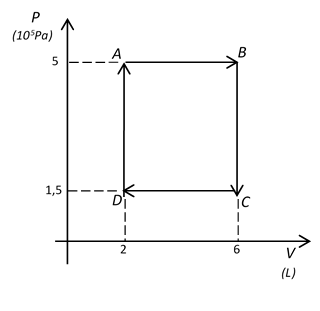
\includegraphics{./capitulo_04/termodin.png}
% \caption{Ejemplificacin de diagrama en blanco y negro.}
% \label{fig:termodin}
% \end{center}
% \end{figure}

% Las tablas deberan contener datos representativos que sinteticen informacin significativa del trabajo, evitando mostrar datos intermedios que pudieran dificultar la interpretacin del mismo.

% Cada tabla debe estar antecedida de un epgrafe que la identifique, enumere y describa brevemente.

% Cada tabla debe ser referenciada al menos una vez, a travs de su nmero, de preferencia antes de que aparezca en el documento, como en este caso (tabla \ref{tab:animales}).

% \begin{table}[H]
% \begin{center}
% \caption{Inventario de animales.}
% \label{tab:animales}
% \begin{tabular}{||l|l|r||}
% \hline
% Especie&Sexo&Cantidad\\
% \hline
% \multirow{2}{*}{palomas}&jvenes&20\\
% &adultas&18\\
% \hline
% \multirow{2}{*}{conejos}&jvenes&5\\
% &adultos&5\\
% \hline
% \multirow{2}{*}{gallinas}&jvenes&50\\
% &adultas&50\\
% \hline
% \multicolumn{2}{||c|}{Total}&148\\
% \hline
% \end{tabular}
% \end{center}
% \end{table}

% Otro ejemplo de tabla en el cual se observa el empleo de color, adems de la combinacin de columnas se observa en la tabla \ref{tab:color}

% \begin{table}[H]
% \begin{center}
% \caption{Clasificacin de la muestra, por edad.}
% \label{tab:color}
% \begin{tabular}{|c|cccc|}
% \hline
% \multirow{2}{*}{\cellcolor[rgb]{0.4,0.8,0.5}} &  \multicolumn{4}{>{\cellcolor[rgb]{0.4,0.8,0.9}}c|}{Tamao de las muestras} \\ 
% \cellcolor[rgb]{0.4,0.8,0.5}Edad&\cellcolor[rgb]{0.4,0.8,0.9} San Lorenzo &\cellcolor[rgb]{0.4,0.8,0.9} Asuncin &\cellcolor[rgb]{0.4,0.8,0.9} Villarrica &\cellcolor[rgb]{0.4,0.8,0.9} Encarnacin \\
% \hline
% e$<$20 &  93 &  74 &  68 & 87 \\
% 19$<$e$<$40 &  52 &  48 &  69 & 70 \\
% 39$<$e$<$60 &  47 &  85 &  81 & 64 \\
% 59$<$e$<$80 &  28 &  36 &  16 & 23 \\
% 79$<$e &  9 &  5 &  6 & 12 \\
% \hline 
% \end{tabular}
% \end{center}
% \end{table}

% Aveces, como en el caso de la tabla \ref{tab:color}, el cdigo se vuelve bastante complejo que resulta engorroso obtener en tiempo razonable la apariencia esperada de la tabla. En esos casos; es posible elaborar la tabla en entorno diferente a Latex; grabarla como imagen png, o jpg, o pdf; e insertarla enmascarada como tabla para ser contada como una de ellas por el contador de tablas: esto se logra con incluir la imagen dentro del entorno ``table'', como se ejemplifica con la tabla \ref{tab:tabla_word} que sigue.

% \begin{table}[H]
% 	\begin{center}
% 		\caption{Imagen de tabla, en reemplazo de la tabla anterior.}
% 		\label{tab:tabla_word}
% 		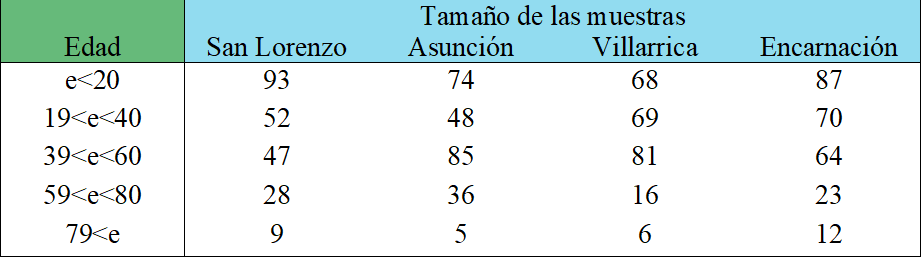
\includegraphics[scale=.65]{./capitulo_04/tabla_word.png}
% 	\end{center}
% \end{table}


% \fancyhead{}
\fancyfoot{}
\cfoot{\thepage}

\lhead{Discusión}

\chapter{Discusión}

% En este captulo, que tambin suele denominarse ``Conclusiones'', se derivan las conclusiones, se explicitan recomendaciones para otros estudios (por ejemplo, sugerir nuevas preguntas, muestras, instrumentos, lneas de investigacin, etc.) y se indica lo que sigue y lo que debe hacerse. Se analiza la posibilidad de extender los resultados a una poblacin mayor que la del estudio. Se evalan las implicaciones, se establece la manera como se respondieron las preguntas de investigacin, si se cumplieron o no los objetivos, se relacionan los resultados con los estudios existentes (vincular con el marco terico y sealar si los resultados coinciden o no con la literatura previa, en qu s y en qu no). Se reconocen las limitaciones de la investigacin, se destaca la importancia y significado de todo el estudio y la forma como encaja en el conocimiento disponible. Se explican los resultados inesperados y cuando no se verificaron las hiptesis es necesario sealar o al menos especular sobre las razones. Recordar que no se deben repetir aqu los resultados sino que se los debe interpretar. La discusin debe redactarse de tal manera que se facilite la toma de decisiones respecto de una teora, un curso de accin o una problemtica. Resumiendo, este captulo puede ser conceptualmente y dividido en al menos tres secciones, como se ilustra a continuacin.

\section{Logros alcanzados}
% Descripcin de los principales descubrimientos obtenidos como producto de la interpretacin de los resultados de la investigacin.
\section{Solución del problema de investigacin}
% Aqu se realiza la discusin propiamente dicha, respondiendo al problema planteado e indicando el nivel de satisfaccin de la solucin lograda.
\section{Sugerencias para futuras investigaciones}
% Todo trabajo de investigacin, genera invariablemente como producto colateral, otras interrogantes que suelen ameritar seguir con la investigacin. Esto es derivado del caracter abierto, \textit{i.e.}, inacabado, del conocimiento cientfico. En esta seccin se acostumbra hacer referencia a posibles seguimientos de la investigacin indicando las interrogantes que conforman nuevos problemas pasibles de ser indagados.   

\backmatter

\cleardoublepage
\addcontentsline{toc}{chapter}{Glosario}
\printglossary

\addcontentsline{toc}{chapter}{Anexos}

\cleardoublepage
\fancyhead{}
\fancyfoot{}
\cfoot{\thepage}

\lhead{Anexo.}
%\rhead{\today}
%\rfoot{\thepage}

\chapter{Anexo.}

Exportación de Python  e importación en javascript del modelo

Pasos para exportar el modelo para su utilización con la librería tensorflow js



\begin{figure}[H]
    \begin{center}
        \begin{subfigure}{0.28\textwidth}
            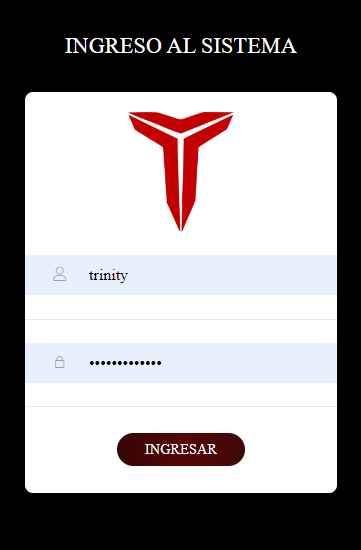
\includegraphics[width=\linewidth]{./sistema/login.png}
            \caption{Interfaz de inicio}
        \end{subfigure}
        \hspace{0.05\textwidth}
        \begin{subfigure}{0.62\textwidth}
            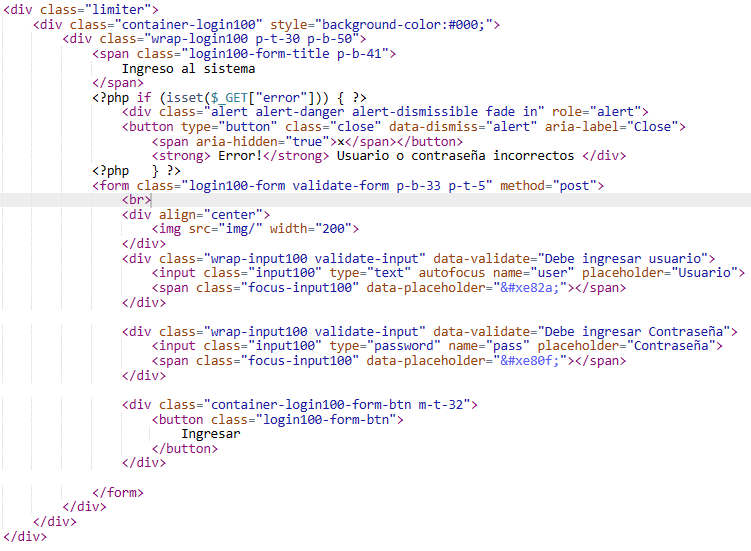
\includegraphics[width=\linewidth]{./sistema/codigo_login.png}
            \caption{Código de inicio de sesión del sistema}
        \end{subfigure}
        \caption{Login del sistema}
        \label{fig:login}
    \end{center}
\end{figure}

Este script PHP se utiliza para la autenticación de usuarios en un sistema web, empleando PHP y MySQL para gestionar la base de datos de usuarios. También se hace uso de tecnologías web como HTML, CSS. para el diseño del formulario de inicio de sesión. El script verifica las credenciales ingresadas por el usuario y, en caso de ser correctas, inicia una sesión y redirige al usuario a una página específica en función de su nivel de acceso. Si las credenciales son incorrectas, se muestra un mensaje de error.


\begin{figure}[H]
    \begin{center}
      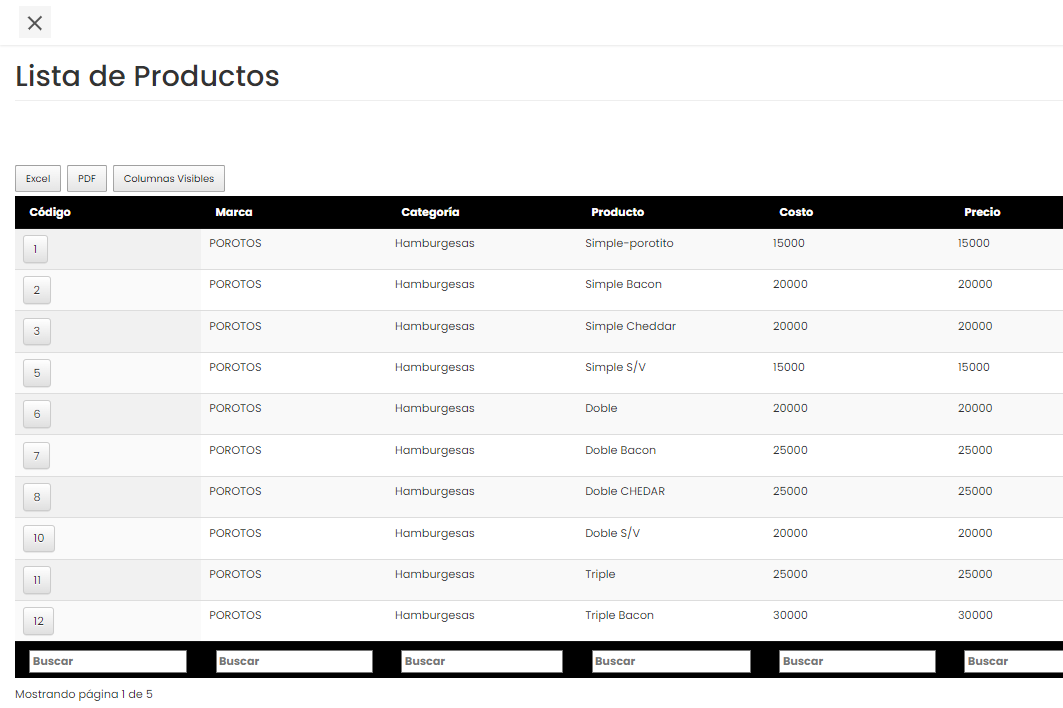
\includegraphics[scale=0.45]{./sistema/lista productos.png}
      \caption{Interfaz productos}
      \label{fig:product}
    \end{center}
  \end{figure}

  \begin{figure}[H]
    \begin{center}
      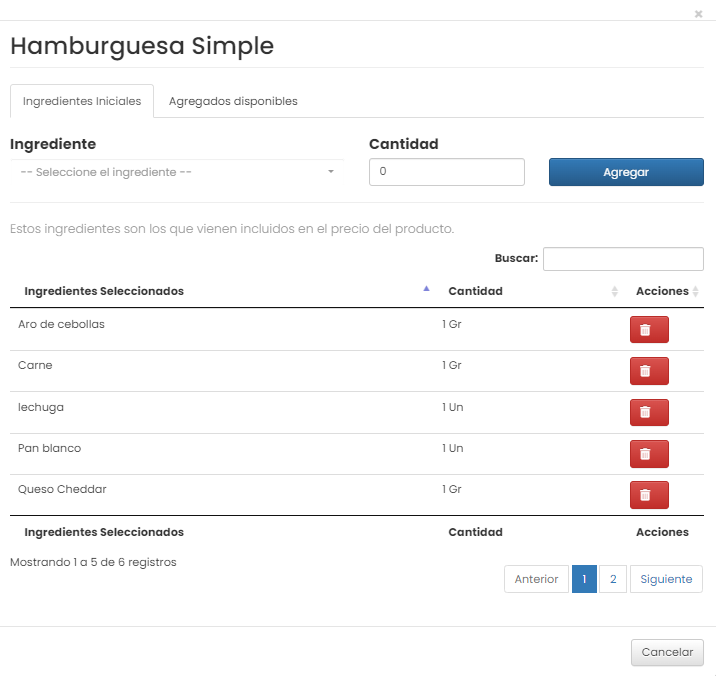
\includegraphics[scale=0.50]{./sistema/ingrediente_de_producto.png}
      \caption{Interfaz de carga de ingredientes}
      \label{fig:product}
    \end{center}
  \end{figure}

  \begin{figure}[H]
    \begin{center}
      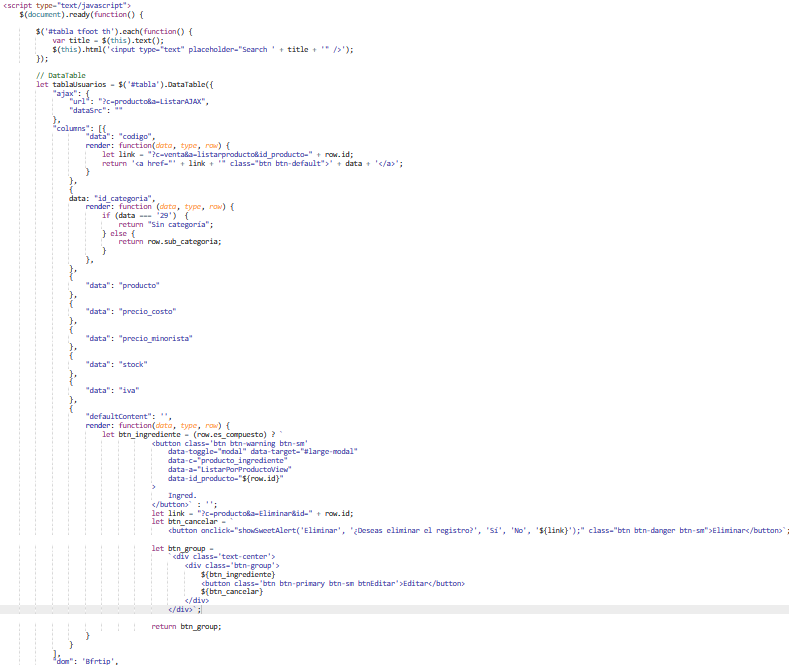
\includegraphics[scale=0.90]{./sistema/producto_codigo.png}
      \caption{Codigo carga de productos e ingresientes}
      \label{fig:product}
    \end{center}
  \end{figure}

El código proporcionado es una combinación de HTML, PHP y JavaScript que se utiliza para crear una página web que muestra una lista de productos. Emplea HTML para estructurar la página, PHP para interactuar con una base de datos y recuperar datos de productos, y JavaScript, incluyendo la biblioteca DataTables, para agregar funcionalidades interactivas a la tabla de productos. La página permite buscar, editar y eliminar productos, y utiliza solicitudes AJAX para comunicarse con el servidor y obtener información sobre los productos. En conjunto, estas tecnologías y herramientas se utilizan para construir una interfaz web dinámica y amigable para la gestión de productos \cite{eguiluz2012introduccion}.

\begin{figure}[H]
    \begin{center}
      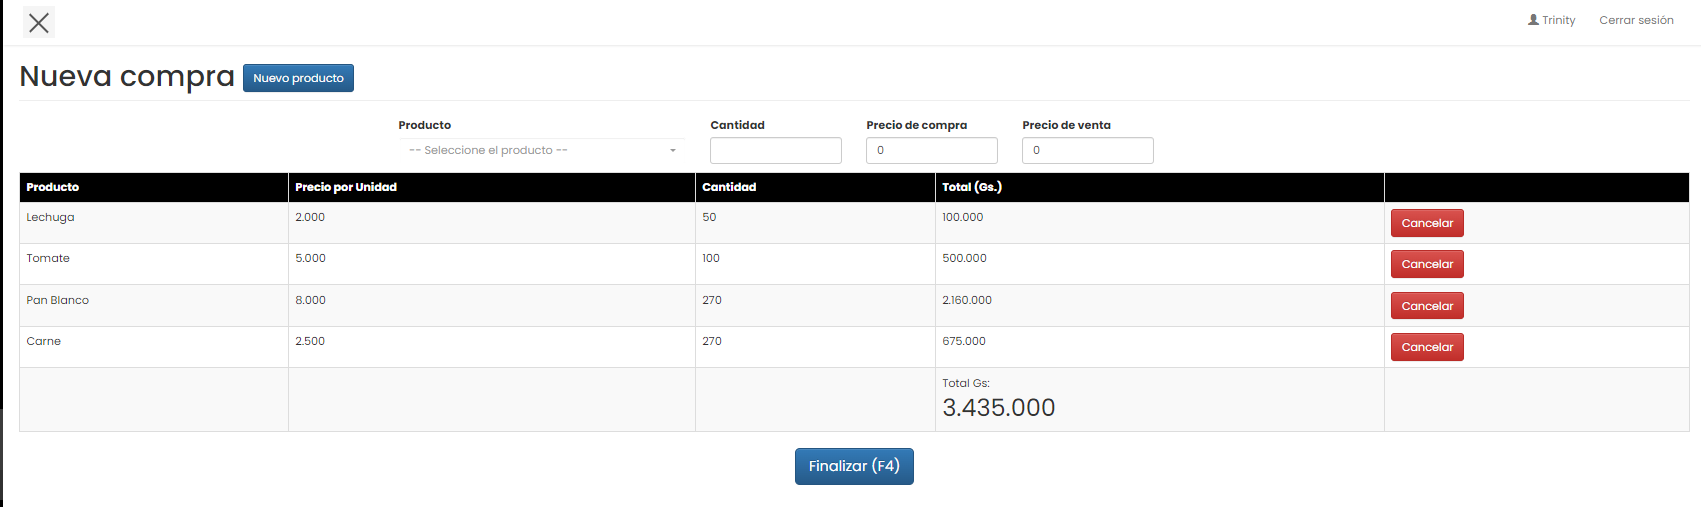
\includegraphics[scale=0.30]{./sistema/compras.png}
      \caption{Interfaz de compras }
      \label{fig:product}
    \end{center}
  \end{figure}
  \begin{figure}[H]
    \begin{center}
      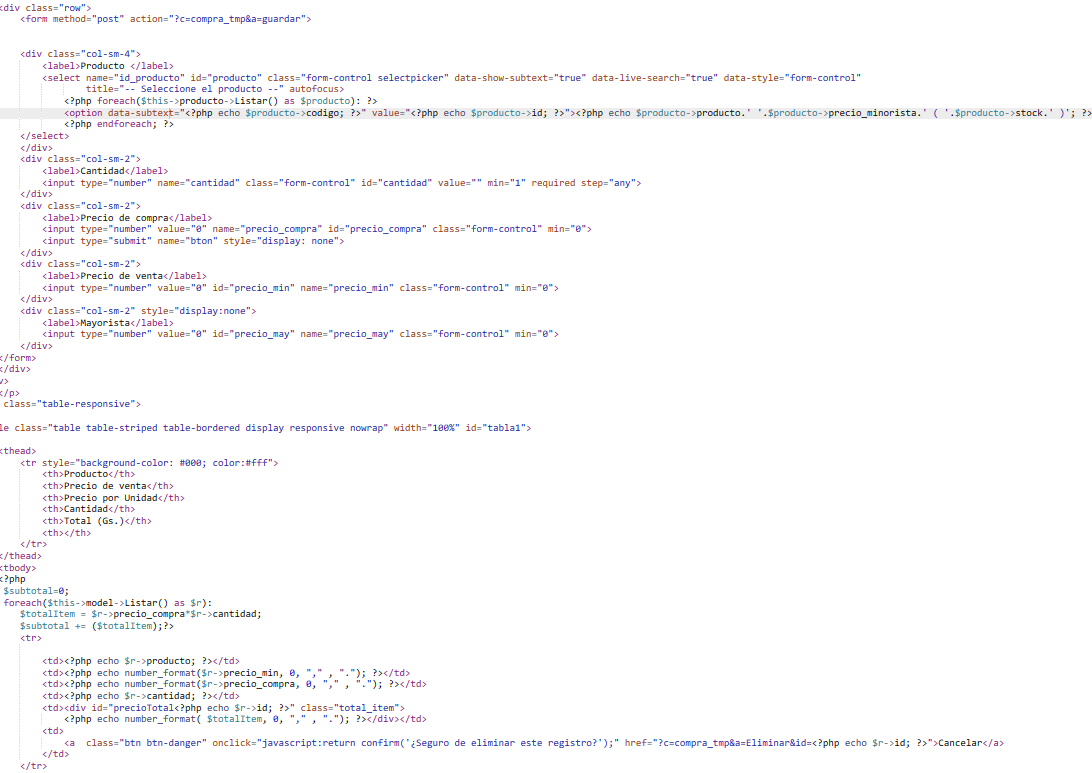
\includegraphics[scale=0.55]{./sistema/codigo_compra.png}
      \caption{Codigo carga de compras }
      \label{fig:product}
    \end{center}
  \end{figure}
  Este código HTML muestra un formulario que permite a los usuarios ingresar detalles de productos, como seleccionar un producto, definir la cantidad, el precio de compra y el precio de venta.

  \begin{figure}[H]
    \begin{center}
      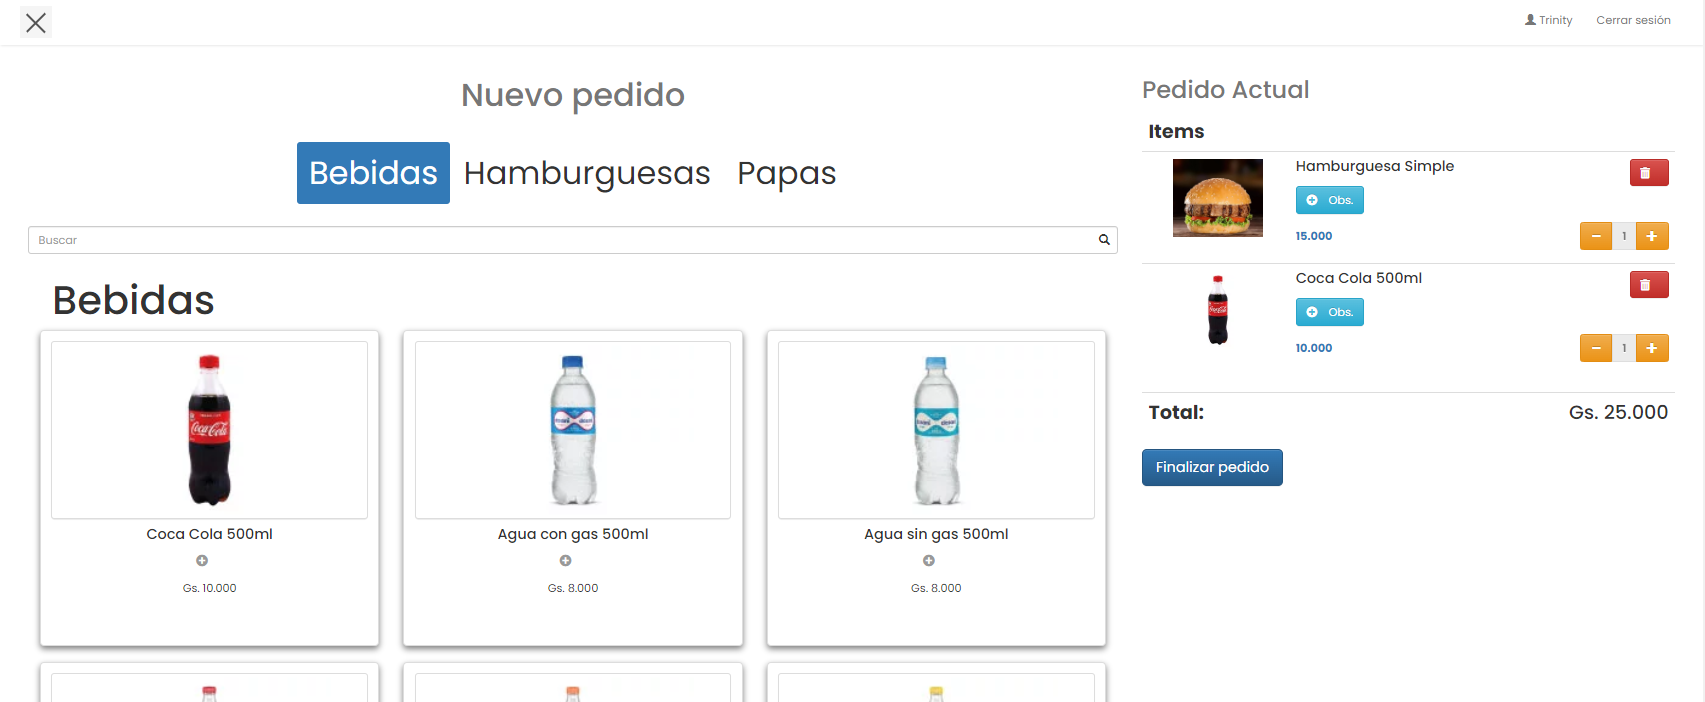
\includegraphics[scale=0.25]{./sistema/nueva_venta.png}
      \caption{Interfaz de ventas}
      \label{fig:product}
    \end{center}
  \end{figure}
  \begin{figure}[H]
    \begin{center}
      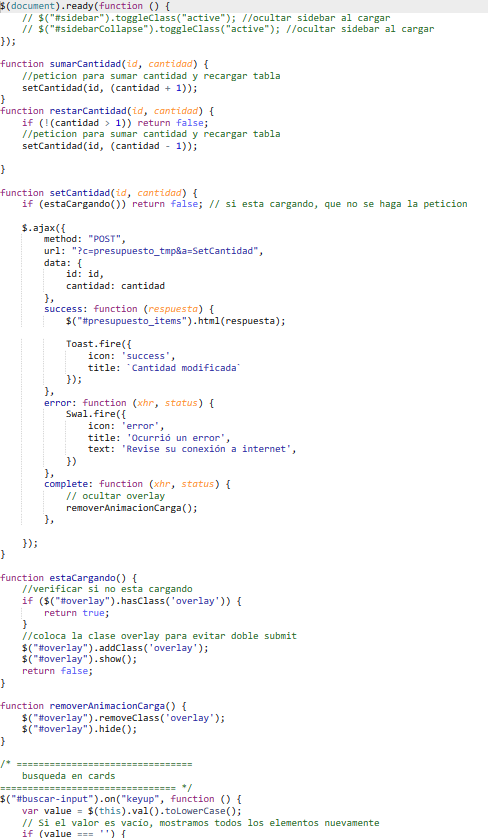
\includegraphics[scale=0.65]{./sistema/codigo_venta.png}
      \caption{Codigo carga de ventas}
      \label{fig:product}
    \end{center}
  \end{figure}

  \begin{figure}[H]
    \begin{center}
      \includegraphics[scale=0.65]{./sistema/lista_predicciones.png}
      \caption{Interfaz de lista de predicciones hechas}
      \label{fig:product}
    \end{center}
  \end{figure}

  \begin{figure}[H]
    \begin{center}
      \includegraphics[scale=0.65]{./sistema/Informe de compra prediccion.png}
      \caption{Informe de predicción de ingredientes a comprar }
      \label{fig:product}
    \end{center}
  \end{figure}




\cleardoublepage
\addcontentsline{toc}{chapter}{Referencias bibliogr\'aficas}

\bibliographystyle{IEEEtran-castellano}
\bibliography{test}
\end{document}

